\documentclass{beamer}    % 14pt je nenujen
\usepackage[T1]{fontenc}
\usepackage[utf8]{inputenc}
\usepackage[slovene]{babel}
\usepackage{pgfpages}           % privat zapiski
\usepackage{amsfonts}
\usepackage{amsmath,amsthm}     % pravilen izpis v "math mode"
%\usepackage{hyperref}
\usepackage{graphicx}           % za slike
\usepackage{tikz}
\usepackage{multicol}
\usepackage{ulem}
\usepackage{bibentry}
\usepackage{bbm}

\usepackage{forest,calc}
\forestset{
  make tab/.style args={#1:#2:#3/#4:#5:#6/#7:#8:#9}{%
    content={%
      \tabcolsep=.6\tabcolsep
      \begin{tabular}{p{\widthof{x}}|p{\widthof{x}}|p{\widthof{x}}}
        #1 & #2 & #3\\\hline#4&#5&#6\\\hline#7&#8&#9
      \end{tabular}}},
  label position r/.initial=right,
  label position b/.initial=below
}

%\hypersetup{hidelinks}

\setbeamertemplate{theorems}[ams style]             % numbered da brez bold 

\setbeameroption{hide notes}                        % samo prosojnice
%\setbeameroption{show only notes}                   % samo zapiski
%\setbeameroption{show notes on second screen=right}  % oboje

\usepackage{palatino}
\usefonttheme{serif}

%\usecolortheme{beetle} %ali beetle morda ali seagull 

\setbeamertemplate{navigation symbols}{} % izklop navigacije
\setbeamertemplate{footline}[frame number]{} % oštevilčenje
\setbeamertemplate{note page}{\pagecolor{yellow!5}\insertnote}

\newtheorem{izrek}{Izrek}
\newtheorem{trditev}[izrek]{Trditev}
\newtheorem{posledica}[izrek]{Posledica}
\newtheorem{definicija}[izrek]{Definicija}
\newtheorem{naloga}[izrek]{Naloga}
\newtheorem{resitev}[izrek]{Naloga}
\newtheorem{hipoteza}[izrek]{Hipoteza}

\author{Tim Kalan \\ \medskip
        \footnotesize Mentor: izr.~prof.~dr. Marjetka Knez}
\institute[FMF]{Fakulteta za matematiko in fiziko}
\title{
    Spodbujevalno učenje pri igranju namiznih iger \\ 
    \large (angl. \textit{Reinforcement learning in board games})}
\date{30. marec 2021} 



\begin{document}

\begin{frame}
    \titlepage
\end{frame}


\begin{frame}
    \frametitle{Napovednik}
    \begin{itemize}
        \item Motivacija, 
        \item problem spodbujevalnega učenja, 
        \item algoritmi, 
        \item namizne igre.
    \end{itemize}
\end{frame}


\begin{frame}
    \frametitle{Umestitev}
    \begin{figure}[b]
        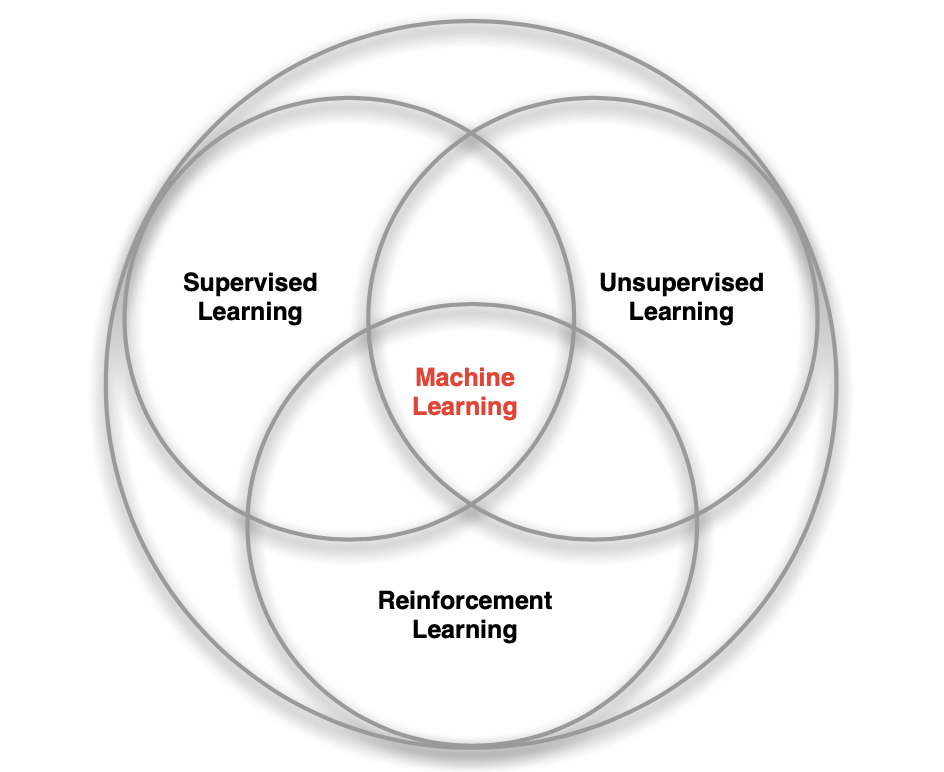
\includegraphics[scale=0.31]{slike/uvod-ml.png}
        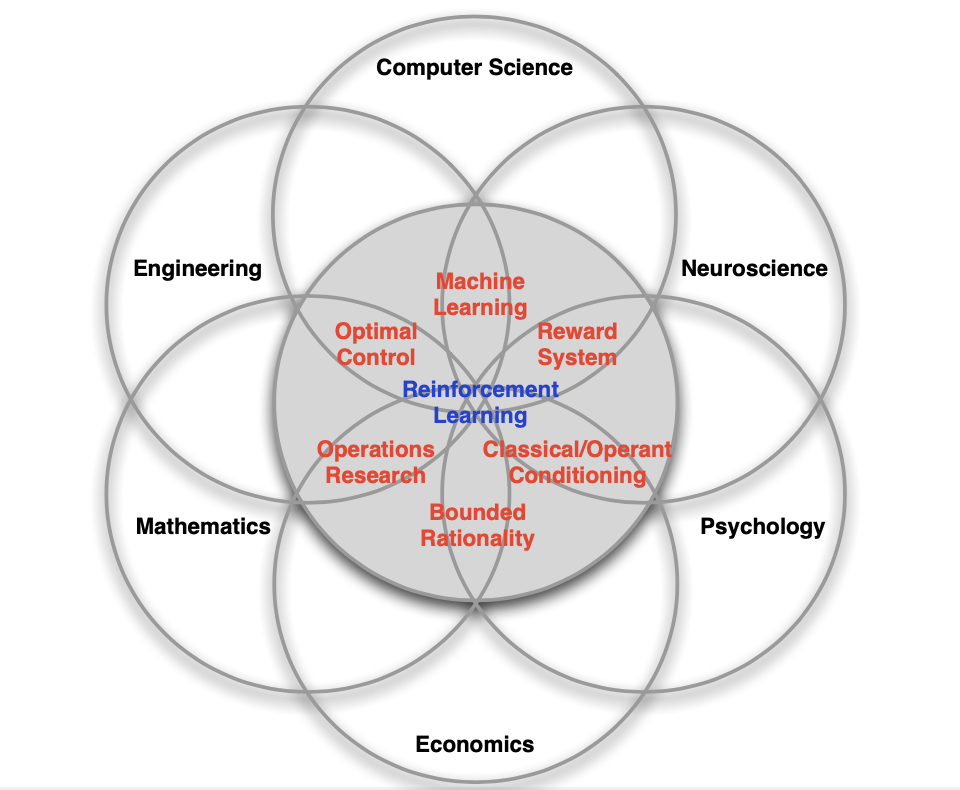
\includegraphics[scale=0.31]{slike/uvod-rl.png}
    \end{figure}
\end{frame}


\begin{frame}
    \frametitle{Motivacija: Instrumentalno pogojevanje}
    \begin{itemize}
        \item Psihološko motivirana podlaga. 
        \item \textbf{Nagrade in kazni}.
    \end{itemize}

    \begin{figure}[b]
        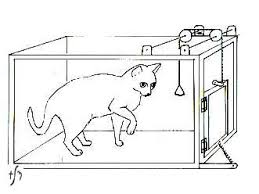
\includegraphics[scale=0.47]{slike/macka.jpg}
        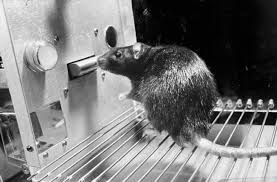
\includegraphics[scale=0.5]{slike/miska.jpg}
    \end{figure}
            
\end{frame}


\begin{frame}
    \frametitle{Okvir}
    \begin{figure}
        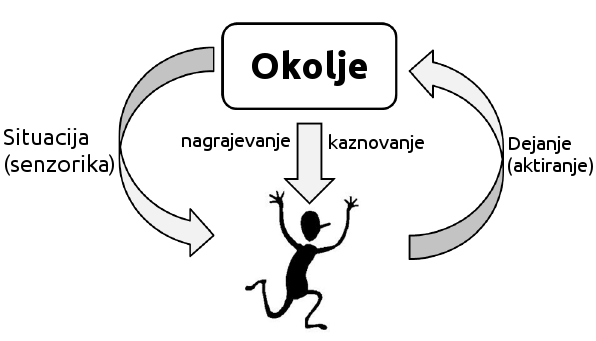
\includegraphics[scale=0.5]{slike/RLloop.png}
    \end{figure}
\end{frame}


\begin{frame}
    \frametitle{Primer 1: robot se uči hoje}
    \begin{itemize}
        \item \textbf{Situacija/Stanje}: položaj v sobi in stanje nog,
        \item \textbf{Nagrada}: $1$ za doseg vrat, $2$ za ključ, $-0.5$ za časovni korak,
        \item \textbf{Okolje}: soba in senzorji, ki govorijo o položaju,
        \item \textbf{Akcija}: Premik noge.
    \end{itemize}
\end{frame}


\begin{frame}[fragile]
    \frametitle{Primer 2: križci in krožci}
    \begin{columns}[T] % align columns
    \begin{column}{.48\textwidth}
    
    \begin{itemize}
        \item \textbf{Situacija/Stanje}: stanje na plošči,
        \item \textbf{Nagrada}: $1$ za zmago, $-1$ za poraz, $x$ za izenačenje/potezo,
        \item \textbf{Okolje}: nasprotnik, plošča, sodnik, nagrajevalec,
        \item \textbf{Akcija}: postavitev $X$ oz. $O$ na ploščo.
    \end{itemize}

    \end{column}%
    \hfill%
    \begin{column}{.48\textwidth}
    
        \begin{forest}
            TTT/.style args={#1:#2}{
              make tab/.expanded=\forestove{content},
              label={\pgfkeysvalueof{/forest/label position #1}:$#2$}
            },
            TTT*/.style={
              make tab=::/::/::,
              content/.expand once=%
              \expandafter\vphantom\expandafter{\romannumeral-`0\forestov{content}},
              draw=none,
              append after command={(\tikzlastnode.north) edge (\tikzlastnode.south)},
              for descendants={before computing xy={l*=1.2}},
            },
            th/.style=thick,
            for tree={node options=draw, inner sep=+0pt, parent anchor=south, child anchor=north}
            [o:x:o/x:x:/x:o:, TTT=r:
                [o:x:o/x:x:o/x:o:, TTT=b:
                    [o:x:o/x:x:o/x:o:x, TTT=b: x]
            ]
                [o:x:o/x:x:/x:o:o, TTT=b:
                    [o:x:o/x:x:x/x:o:o, TTT=b: 1]
            ]
            ]
        \end{forest}

    \end{column}%
    \end{columns}
    \end{frame}


    \begin{frame}
        \frametitle{Ideja}
        \begin{itemize}
            \item Agent ">pade"< v okolje. 
            \item S poskušanjem se nauči pravilnih akcij.
            \item Svoje znanje izkoristi za maksimizacijo nagrade.
        \end{itemize}

        \pause
        \medskip
        
        \begin{hipoteza}[Hipoteza o nagradi]
            Vse cilje je mogoče opisati kot maksimizacijo neke kumulativne numerične 
            nagrade.
        \end{hipoteza}

    \end{frame}


\begin{frame}
    \frametitle{Formalizacija: Markovski proces odločanja 1}
    \begin{definicija}[Markovska veriga]
        Slučajni proces $(S_t)_{t=0}^T$ na končnem verjetnostnem prostoru 
        $(\Omega, \mathcal{F},  P)$ je \textbf{Markovska veriga}, če velja Markovska lastnost
        $$
        P(S_{t+1} = s_{t+1}~|~S_{t} = s_{t}, ..., S_0 = s_0) = P(S_{t+1} = s_{t+1}~|~S_{t} = s_{t})
        $$
    \end{definicija}
    \pause
    \medskip
    \begin{itemize}
        \item Prihodnost je neodvisna od preteklosti, če poznamo sedanjost
        \pause
        \item $p_{ss'} := P(S_{t+1} = s'~|~S_{t} = s) \rightarrow
                \mathcal{P} := [p_{ss'}]_{s,s'\in \mathcal{S} }$, $\mathcal{S}$ 
                je množica stanj
        \item \emph{Markovska veriga} je torej dvojica $(\mathcal{S}, \mathcal{P})$
    \end{itemize}
    
\end{frame}


\begin{frame}
    \frametitle{Formalizacija: Markovski proces odločanja 2}
    \begin{definicija}[Markovski proces nagrajevanja]
        \textbf{Markovski proces nagrajevanja} je nabor 
        $(\mathcal{S}, \mathcal{P}, \mathcal{R}, \gamma)$, kjer je
        \begin{itemize}
            \item $\mathcal{S}$ (končna) množica stanj,
            \item $\mathcal{P}$ prehodna matrika, kjer $\mathcal{P}_{ss'} = P(S_{t+1} = s'~|~S_{t} = s)$,
            \item $\mathcal{R}$ nagradna funkcija $\mathcal{R}_s = E[R_{t+1}~|~S_{t} = s]$,
            \item $\gamma \in [0, 1]$ je diskontni faktor.
        \end{itemize}
    \end{definicija}
\end{frame}


\begin{frame}
    \frametitle{Formalizacija: Markovski proces odločanja 3}
    \begin{definicija}[Markovski proces odločanja]
        \textbf{Markovski proces odločanja (MDP)} je nabor 
        $(\mathcal{S}, \mathcal{A}, \mathcal{P}, \mathcal{R}, \gamma)$, kjer je
        \begin{itemize}
            \item $\mathcal{S}$ (končna) množica stanj,
            \item $\mathcal{A}$ (končna) množica akcij oz. dejanj,
            \item $\mathcal{P}$ prehodna matrika, kjer $\mathcal{P}_{ss'}^a = P(S_{t+1} = s'~|~S_{t} = s,
                    \mathbf{A_t = a})$,
            \item $\mathcal{R}$ nagradna funkcija $\mathcal{R}_s^a = E[R_{t+1}~|~S_{t} = s, 
                    \mathbf{A_t = a}]$,
            \item $\gamma \in [0, 1]$ diskontni faktor.
        \end{itemize}
    \end{definicija}
\end{frame}


\begin{frame}
    \frametitle{Primer: MDP}
    \begin{figure}[b]
        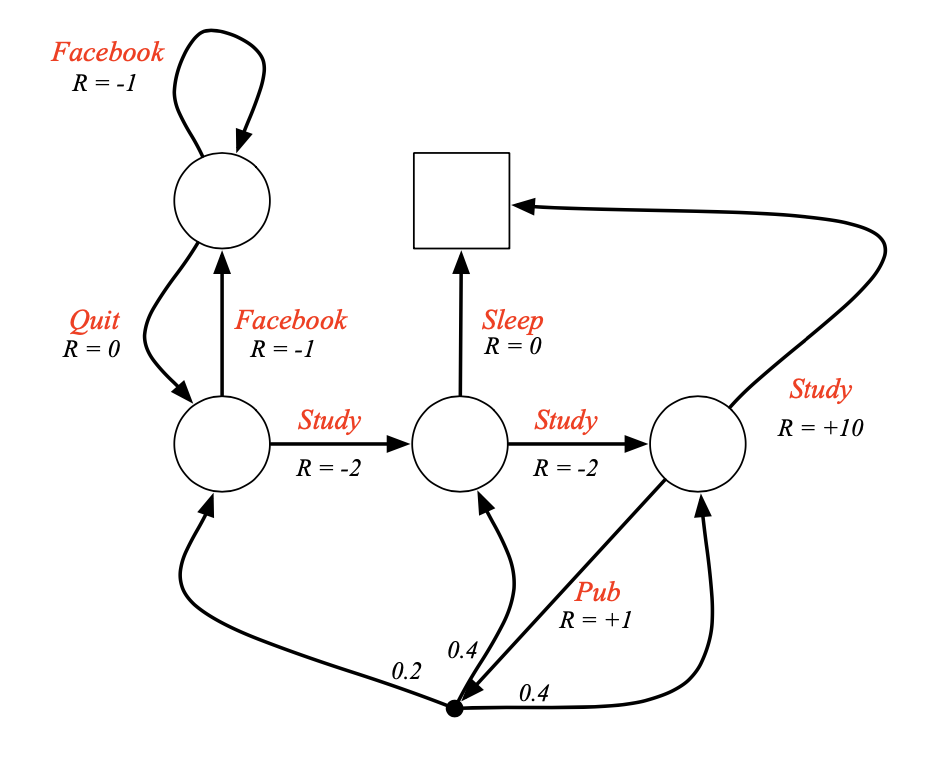
\includegraphics[scale=0.6]{slike/mdp.png}
    \end{figure}
\end{frame}


\begin{frame}
    \frametitle{Agent 1}
    \begin{itemize}
        \item Strategija (angl. \textit{Policy})
        \item Vrednostna funkcija (angl. \textit{Value function})
        \item (Model)
    \end{itemize}
\end{frame}


\begin{frame}
    \frametitle{Agent 2: strategija}
    \begin{definicija}
        \begin{itemize}
            \item \textbf{Deterministična strategija} stanju $s$ priredi akcijo $a$, 
                    $$
                    \pi(s) = a.
                    $$ 
            \item \textbf{Stohastična strategija} za vsako stanje $s$ pove verjetnosti vseh 
                    možnih akcij $a$, 
                    $$
                    \pi(a | s) = P(A_t = a~|~S_t = s).
                    $$
        \end{itemize}
    \end{definicija}
\end{frame}


\begin{frame}
    \frametitle{Agent 3: vrednostna funkcija}
    \begin{definicija}[Povračilo]
        $$
        G_t = R_{t+1} + \gamma R_{t+2} + ... = \sum_{k=0}^\infty \gamma^k R_{t + k + 1}
        $$
    \end{definicija}
    \begin{definicija}[Vrednostna funkcija]
        \begin{itemize}
            \item \textbf{Vrednostna funkcija stanja} je pričakovana vrednost povračila, če se 
                    vedemo skladno s strategijo $\pi$ 
                    $$
                    v_\pi(s) = \mathrm{E} [G_t~|~S_t = s].
                    $$
            \item \textbf{Vrednostna funkcija akcije} je podobna prejšnji, le da sprosti prvo akcijo 
                    $$
                    q_\pi(s, a) = \mathrm{E} [G_t~|~S_t = s, A_t = a].
                    $$
        \end{itemize}
    \end{definicija}
\end{frame}


\begin{frame}
    \frametitle{Primer: strategija in vrednostna funkcija}
    \begin{figure}[b]
        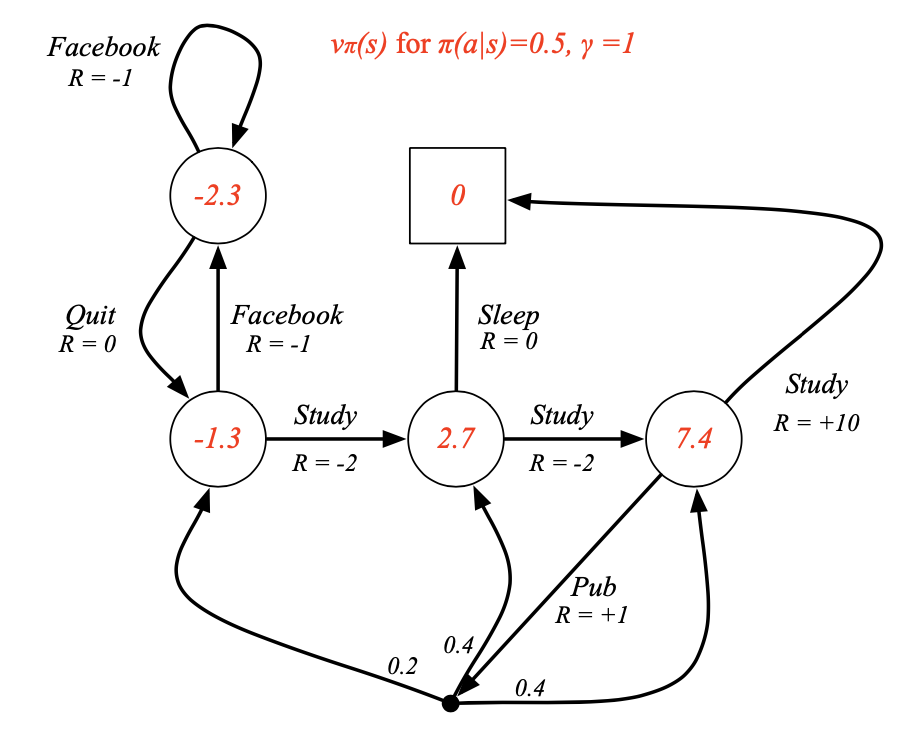
\includegraphics[scale=0.6]{slike/strat-vrednost.png}
    \end{figure}
\end{frame}


\begin{frame}
    \frametitle{Algoritmi}
    \begin{itemize}
        \item Učenje prek strategije ali \textbf{vrednostne funkcije}. 
        \item Celoten problem je \textbf{načrtovanje}:
        \begin{itemize}
            \item Napovedovanje - ugotvaljanje vrednosti.
            \item Upravljanje - iskanje optimalne strategije. 
        \end{itemize}
    \end{itemize}
\end{frame}


\begin{frame}
    \frametitle{Algoritmi: dinamično programiranje 1}
    \begin{itemize}
        \item Poznamo $\mathcal{P}_{ss'}^a$ in $\mathcal{R}_s^a$, 
        \item Bellmanove enačbe, 
        \item vrednostna funkcija - ponovna uporaba rešitev,  
        \begin{align*}
            v_\pi(s) &= \mathrm{E} [G_t~|~S_t = s] \\
                 &= \mathrm{E} [\sum_{k=0}^\infty \gamma^k R_{t + k + 1}~|~S_t = s] \\
                 &= \mathrm{E} [R_{t+1} + \sum_{k=1}^\infty \gamma^k R_{t + k + 1}~|~S_t = s] \\
                 &= \mathrm{E} [R_{t+1} + \gamma(\sum_{k=1}^\infty \gamma^{k-1} R_{t + k + 1})~|~S_t = s] \\
                 &= \mathrm{E} [R_{t+1} + \gamma G_{t+1}~|~S_t = s] \\
                 &= \mathrm{E} [R_{t+1} + \gamma v_\pi(S_{t+1})~|~S_t = s].
        \end{align*}
    \end{itemize}
\end{frame}


\begin{frame}
    \frametitle{Algoritmi: dinamično programiranje 2}
    \begin{figure}
        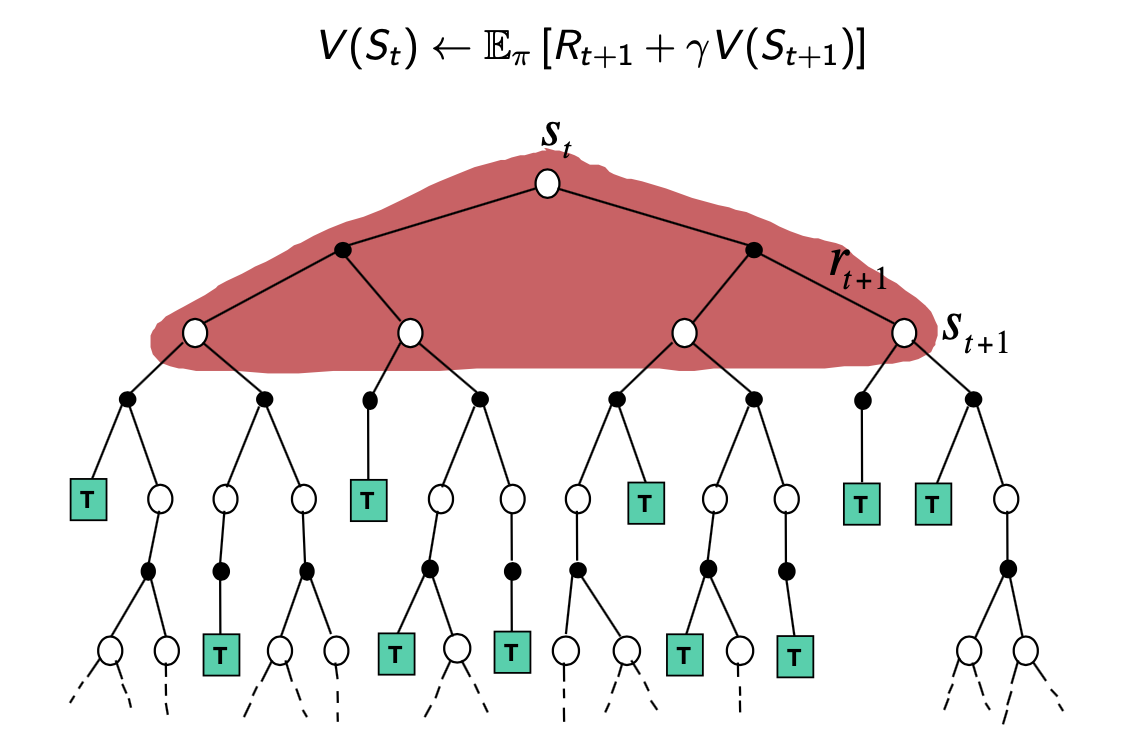
\includegraphics[scale=0.45]{slike/backup-dp.png}
    \end{figure}
\end{frame}


\begin{frame}
    \frametitle{Algoritmi: Monte Carlo 1}
    \begin{itemize}
        \item Nepoznan epizodični MDP, 
        \item problem napovedovanja, 
        \item empirično povračilo, 
        \item štejemo obiske stanj.
    \end{itemize}
\end{frame}


\begin{frame}
    \frametitle{Algoritmi: Monte Carlo 2}
    \begin{itemize}
        \item Ob \textbf{prvem} obisku stanja $s$: 
        \begin{align*}
            N(s) &\leftarrow N(s) + 1 \\
            S(s) &\leftarrow S(s) + G_t
        \end{align*}
        \item Po koncu učenja: 
        $$
        V(s) \leftarrow S(s) / N(s)
        $$
       \item Pomni: Računanje povprečja zaporedja $(X_i)_{i \in \mathbb{N}}$
       $$
       \mu_k = \frac{1}{k} \sum_{j=1}^k X_j = \mu_{k-1} + \frac{1}{k} (X_k - \mu_{k-1})
       $$
       \item Inkrementalni Monte Carlo:
       $$
       V(S_t) \leftarrow V(S_t) + \frac{1}{N(t)} (G_t - V(S_t))
       $$
    \end{itemize}
\end{frame}


\begin{frame}
    \frametitle{Algoritmi: Monte Carlo 3}
    \begin{itemize}
        \item Inkrementalni Monte Carlo:
                %$$
                %V(s) \leftarrow V(s) + \alpha (G_t - V(S_t)).
                %$$
                \begin{figure}[b]
                    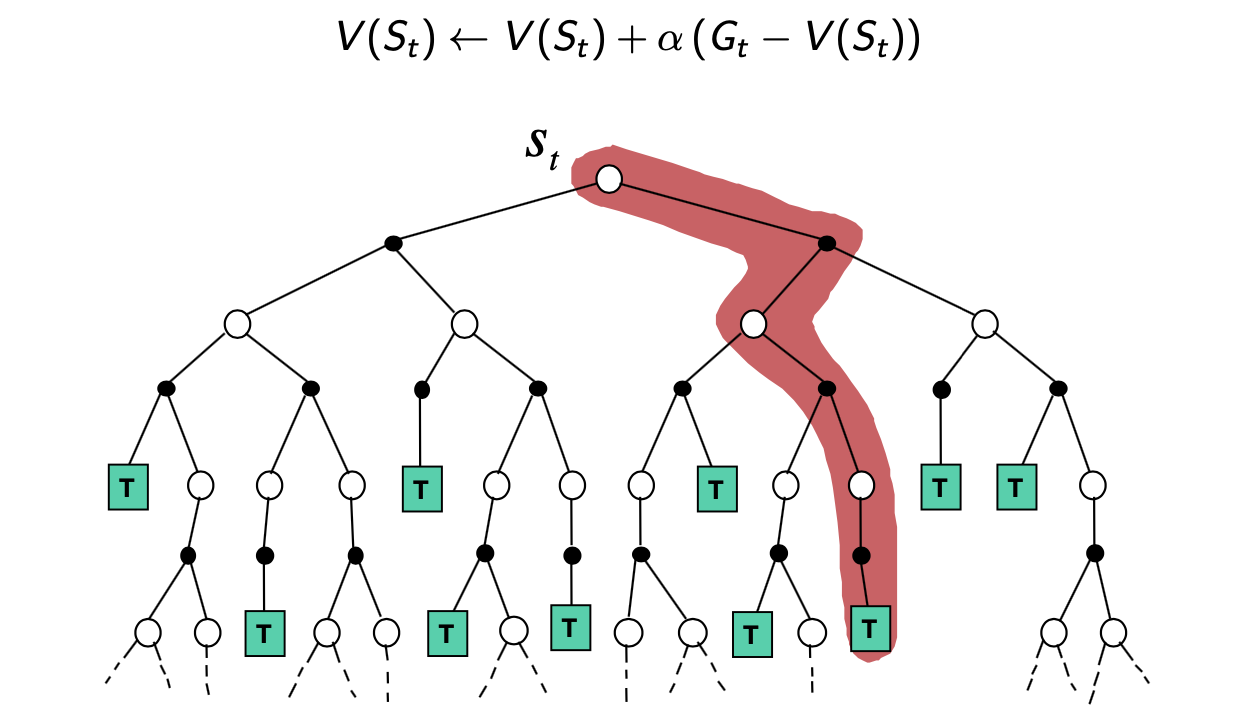
\includegraphics[scale=0.45]{slike/backup-mc.png}
                \end{figure}
        \item Splošni obrazec: 
                $$
                \textit{nova ocena} \leftarrow \textit{stara ocena} + \textit{korak } 
                (\textit{tarča} - \textit{stara ocena}).
                $$
    \end{itemize}
\end{frame}


\begin{frame}
    \frametitle{Algoritmi: TD($0$)}
    \begin{itemize}
        \item Učenje s časovno razliko.
        \item \textit{Bootstrapping}. 
        \item Ne potrebujejo povračila.
        \item $G_t \approx R_{t+1} + \gamma V(S_{t+1})$.
    \end{itemize}

    %\medskip
    %$$
    %V(S_t) \leftarrow V(S_t) + \alpha (R_{t+1} + \gamma V(S_{t+1}) - V(S_t)).
    %$$
    \begin{figure}[b]
        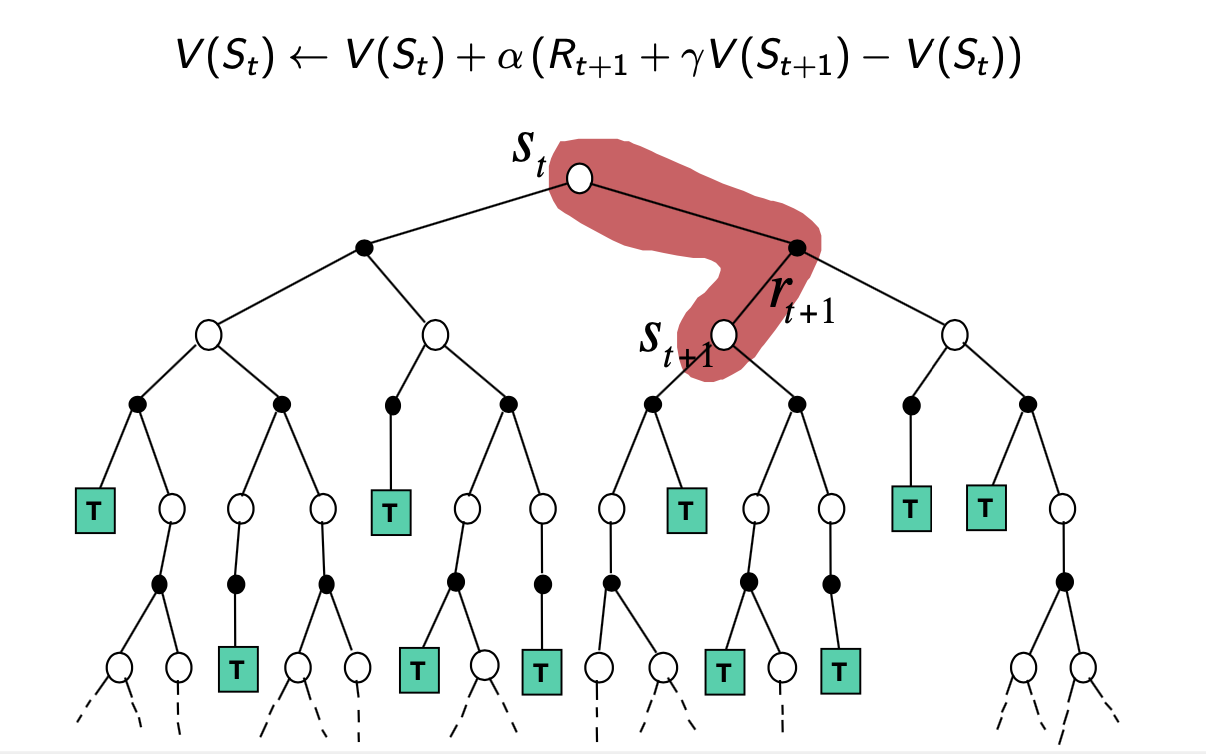
\includegraphics[scale=0.45]{slike/backup-td.png}
    \end{figure}
\end{frame}


\begin{frame}
    \frametitle{Algoritmi: TD($\lambda$) 1}
    \begin{itemize}
        \item Povezava med MC in TD($0$).
        \item $G_t^{(n)} = R_{t+1} + \dots + \gamma^{n-1} R_{t+n} + \gamma^n V(S_{t+1}).$
        \item Povprečenje različnih $G_t^{(n)}$: $G_t^\lambda = (1 - \lambda) \sum_{n=1}^\infty 
                                                 \lambda^{(n-1)} G_t^{(n)}.$
    \end{itemize}

    \medskip
    \medskip
    \medskip
    TD($\lambda$) s \textbf{pogledom naprej}: 
    $$
    V(S_t) \leftarrow V(S_t) + \alpha (G_t^\lambda - V(S_t)).
    $$
    \begin{figure}[b]
        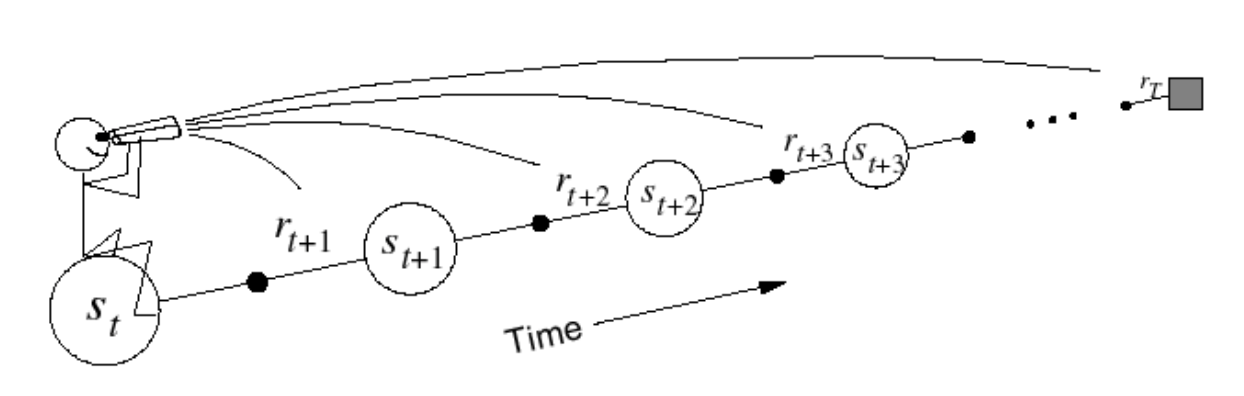
\includegraphics[scale=0.45]{slike/pogled-naprej.png}
    \end{figure}
\end{frame}


\begin{frame}
    \frametitle{Algoritmi: TD($\lambda$) 2}
    \begin{itemize}
        \item \textbf{Sledi upravičenosti} (angl. \textit{eligibility traces}):
        \begin{align*}
            E_0(s) &= 0, \\
            E_t(s) &= \gamma \lambda E_{t-1}(s) + \mathbbm{1}(S_t = s),
        \end{align*}
    \begin{figure}
        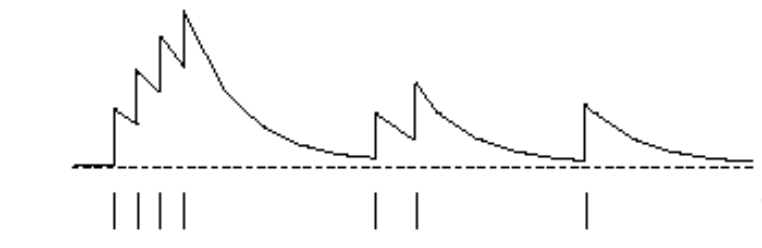
\includegraphics[scale=0.25]{slike/et.png}
    \end{figure}
        \item $\delta_t = R_{t+1} + \gamma V(S_{t+1}) - V(S_t).$
    \end{itemize}

    \medskip
    \medskip
    \medskip
    TD($\lambda$) s \textbf{pogledom nazaj}: 
    $$
    V(s) \leftarrow V(s) + \alpha \delta_t E_t(s).
    $$
    \begin{figure}[b]
        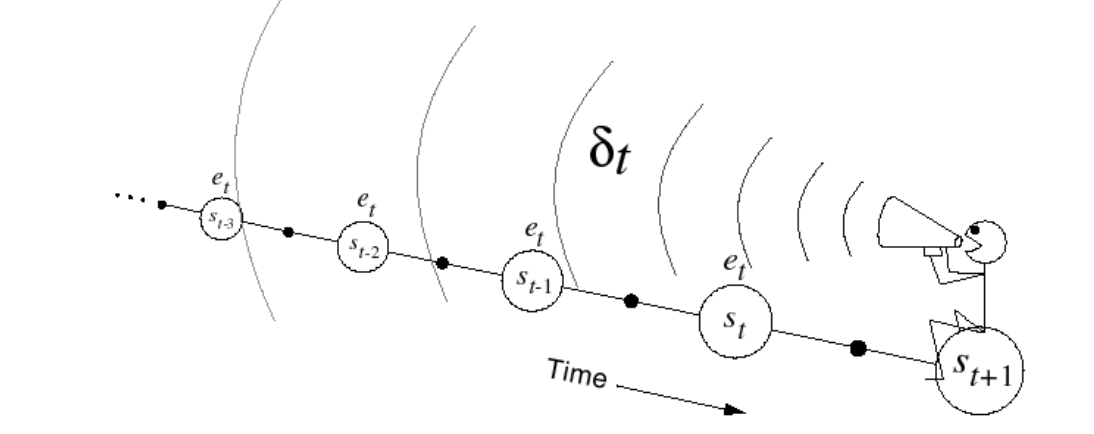
\includegraphics[scale=0.35]{slike/pogled-nazaj.png}
    \end{figure}
\end{frame}


\begin{frame}
    \frametitle{Spreminjanje strategije - upravljanje}
    \begin{itemize}
        \item Potrebujemo vrednostno funkcijo akcij. 
        \item raziskovanje in izkoriščanje.
        \item $\epsilon$-požrešna izbira akcij:
        \begin{equation*}
            \pi(a|s) = \begin{cases}
                        \epsilon / m + 1 - \epsilon & \text{če } a^* = \text{arg}\max_{a \in 
                            \mathcal{A}} Q(s, a) \\
                            \epsilon / m & \text{sicer}
                       \end{cases}
        \end{equation*}
    \end{itemize}
    \begin{figure}
        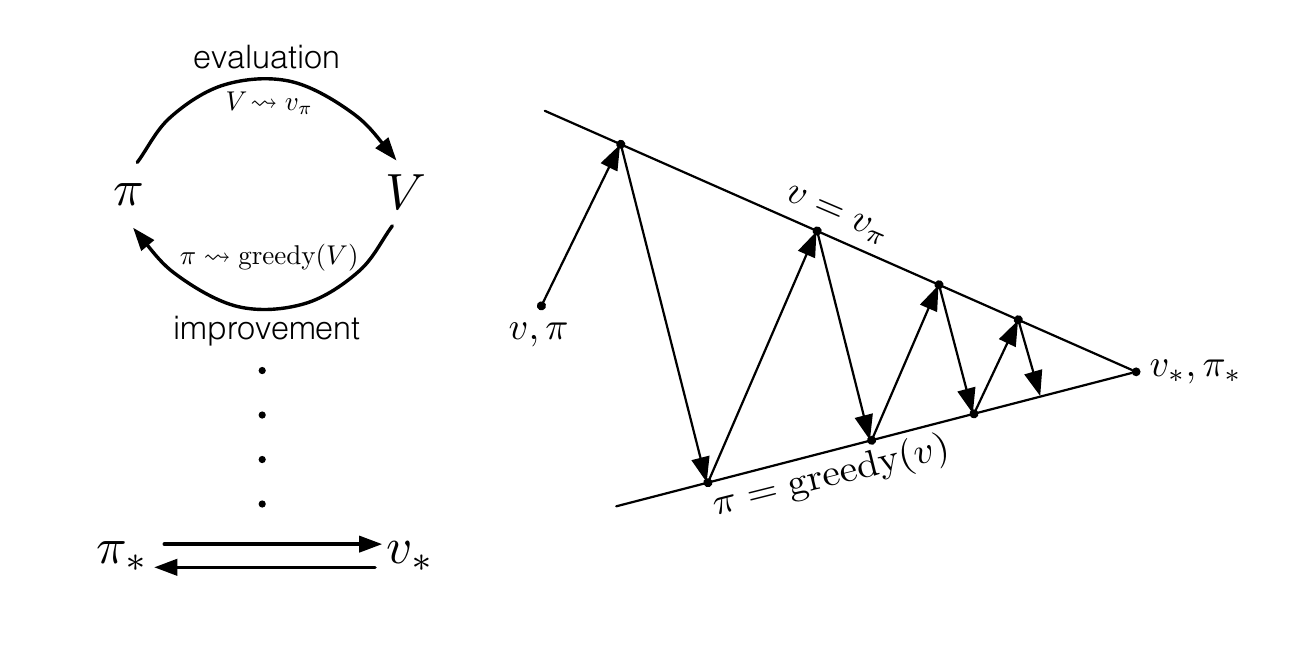
\includegraphics[scale=0.2]{slike/policy-iteration.png}
    \end{figure}
\end{frame}


\begin{frame}
    \frametitle{Konvergenca}
    \begin{itemize}
        \item \textbf{GLIE}:
                \begin{align*}
                    \lim_{k \rightarrow \infty} N_k(s, a) &= \infty, \\
                    \lim_{k \rightarrow \infty} \pi_k(a|s) &= \mathbbm{1}(a =
                             \text{arg}\max_{a' \in \mathcal{A}}Q_k(s, a')).
                \end{align*}
        \item \textbf{Robbins-Monro} zaporedje \textit{korakov} $\alpha_t$:
                \begin{align*}
                    \sum_{t=1}^\infty \alpha_t &= \infty, \\
                    \sum_{t=1}^\infty \alpha_t^2 &< \infty
                \end{align*}
    \end{itemize}
\end{frame}


\begin{frame}
    \frametitle{Težave}
    \begin{itemize}
        \item Veliki MDP-ji:
                \begin{itemize}
                    \item Križci in krožci: $3^9$ / $4578$ / $765$ stanj, 
                    \item Štiri v vrsto: $4.531.985.219.092$ stanj,
                    \item Šah: približno $10^{46}$ stanj, 
                    \item Go: $10^{170}$ stanj, 
                \end{itemize}
        \item Vsi zgornji algoritmi so tabelarični.
        \item Počasno učenje.
    \end{itemize}
\end{frame}


\begin{frame}
    \frametitle{Aproksimacija}
    \begin{itemize}
        \item Linearna Aproksimacija.
        \item Nevronske mreže.
    \end{itemize}
    \begin{figure}
        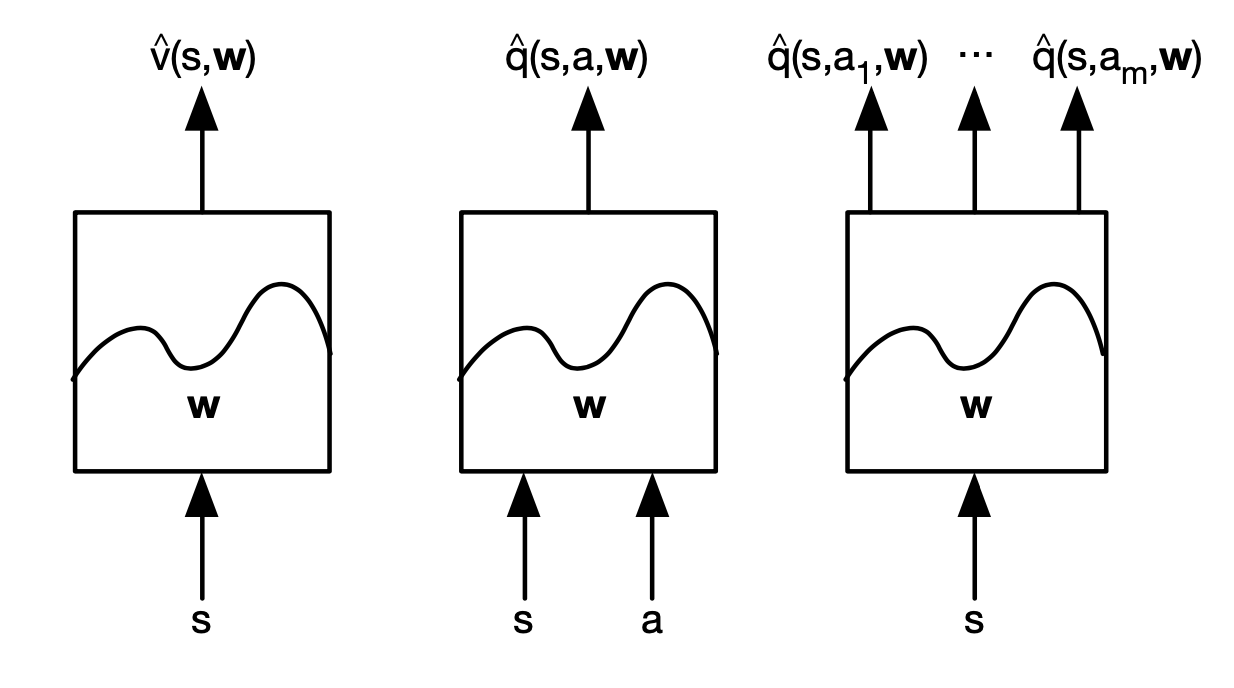
\includegraphics[scale=0.5]{slike/aproksimacija.png}
    \end{figure}
\end{frame}


\begin{frame}
    \frametitle{Namizne igre: posebnosti}
    \begin{itemize}
        \item ">Postanja"<. 
        \item Trening: 
                \begin{itemize}
                    \item Fiksiran nasprotnik, 
                    \item naključni nasprotnik,
                    \item samoigra.
                \end{itemize}
        \item Več agentov: $\pi = \langle \pi^1, \pi ^2 \rangle$.
        \item Iskanje.
        
        \medskip
        \medskip
        $$
        v_*(s) = \max_{\pi^1} \min_{\pi^2} v_\pi(s)
        $$
    \end{itemize}
\end{frame}


\begin{frame}
    \frametitle{m,n,k-igra}
    \begin{itemize}
        \item Dva igralca, vsota nič, ekstenzivna,
        \item $m \times n$ plošča, 
        \item $k$ v vrsto, 
        \item pravila križcev in krožcev (3,3,3-igra),
        \item prilagoditve: gravitacija.
    \end{itemize}
\end{frame}


\begin{frame}
    \frametitle{3,3,3-igra 1}
    \begin{figure}
        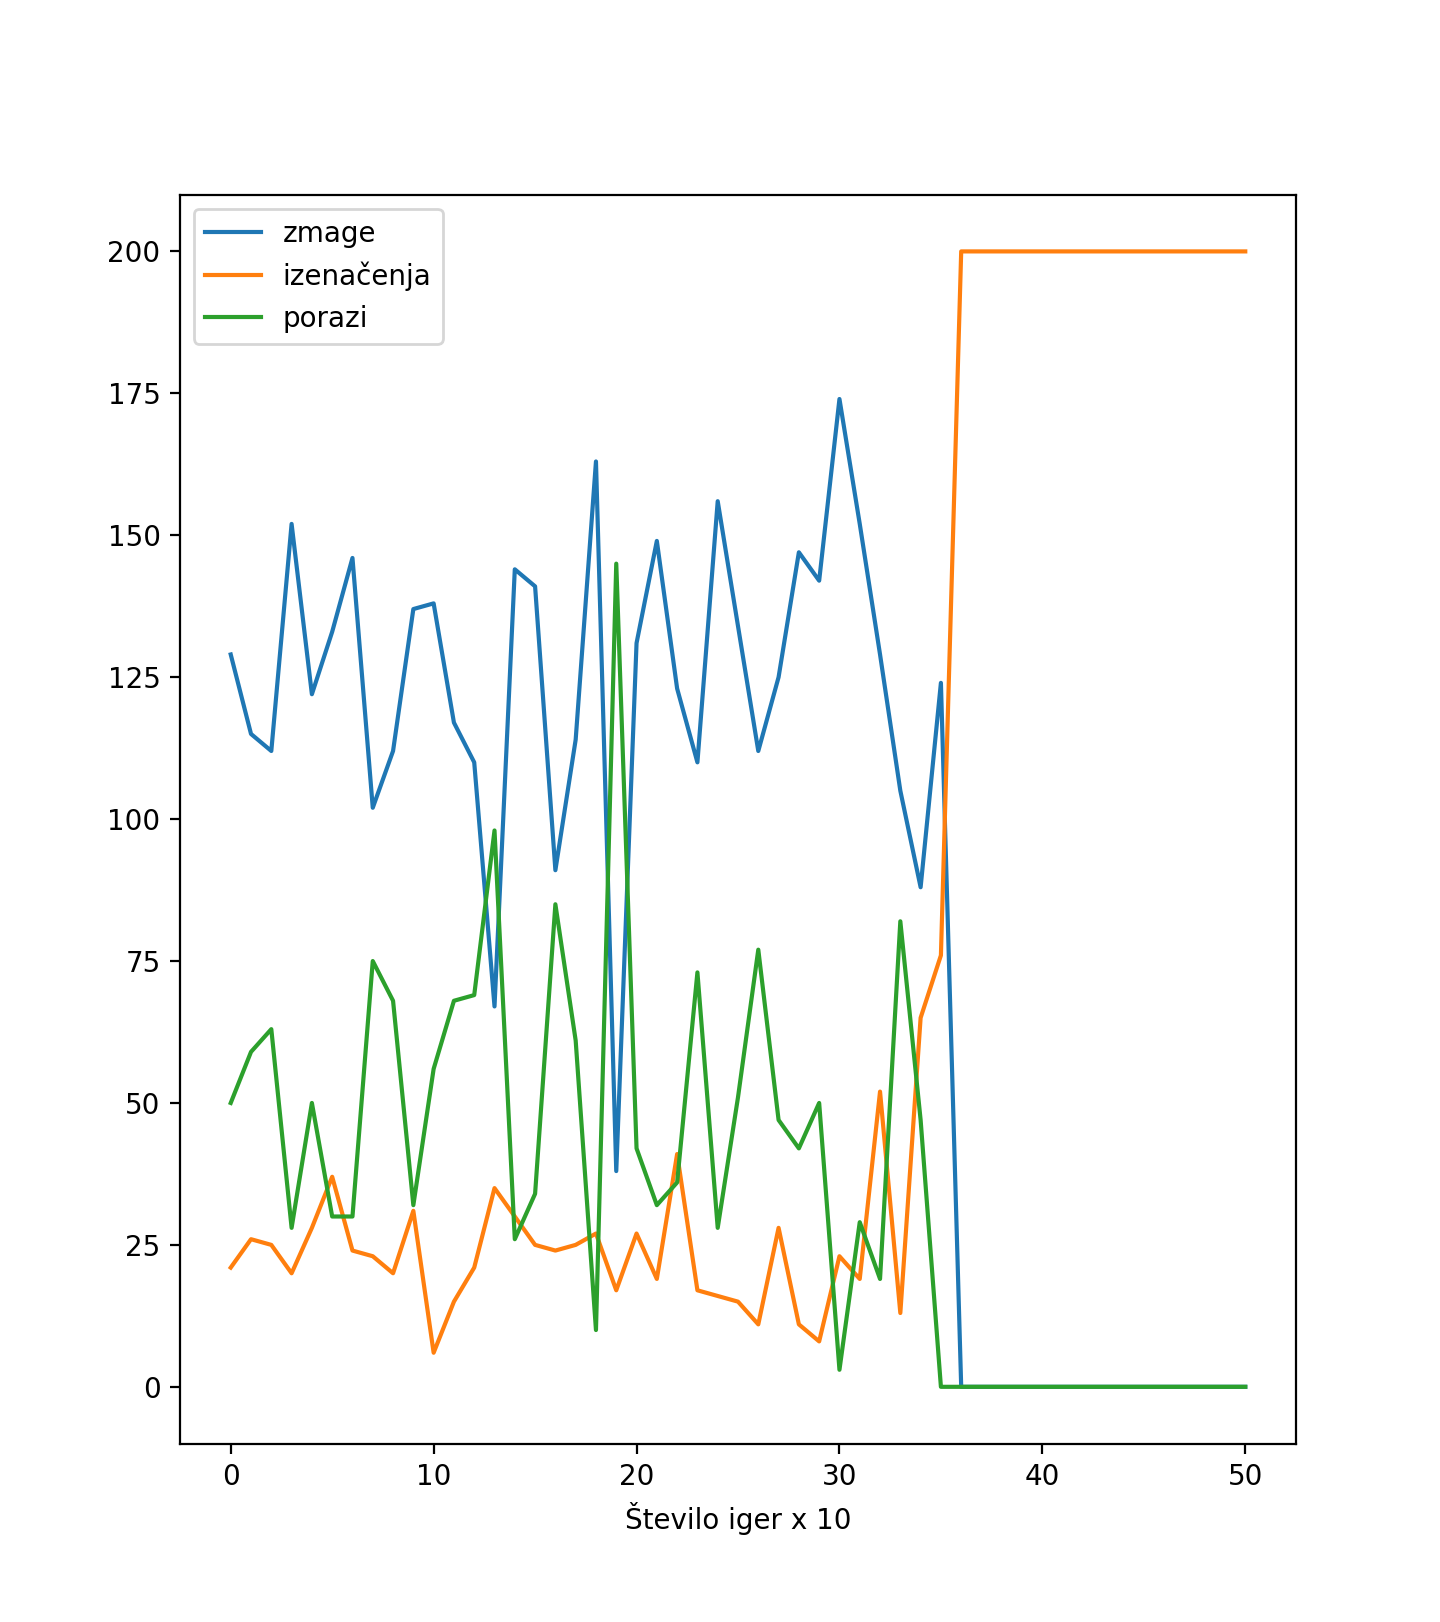
\includegraphics[scale=0.4]{slike/ag-ag_500_200_10.png}
    \end{figure}
\end{frame}


\begin{frame}
    \frametitle{3,3,3-igra 2}
    \begin{figure}
        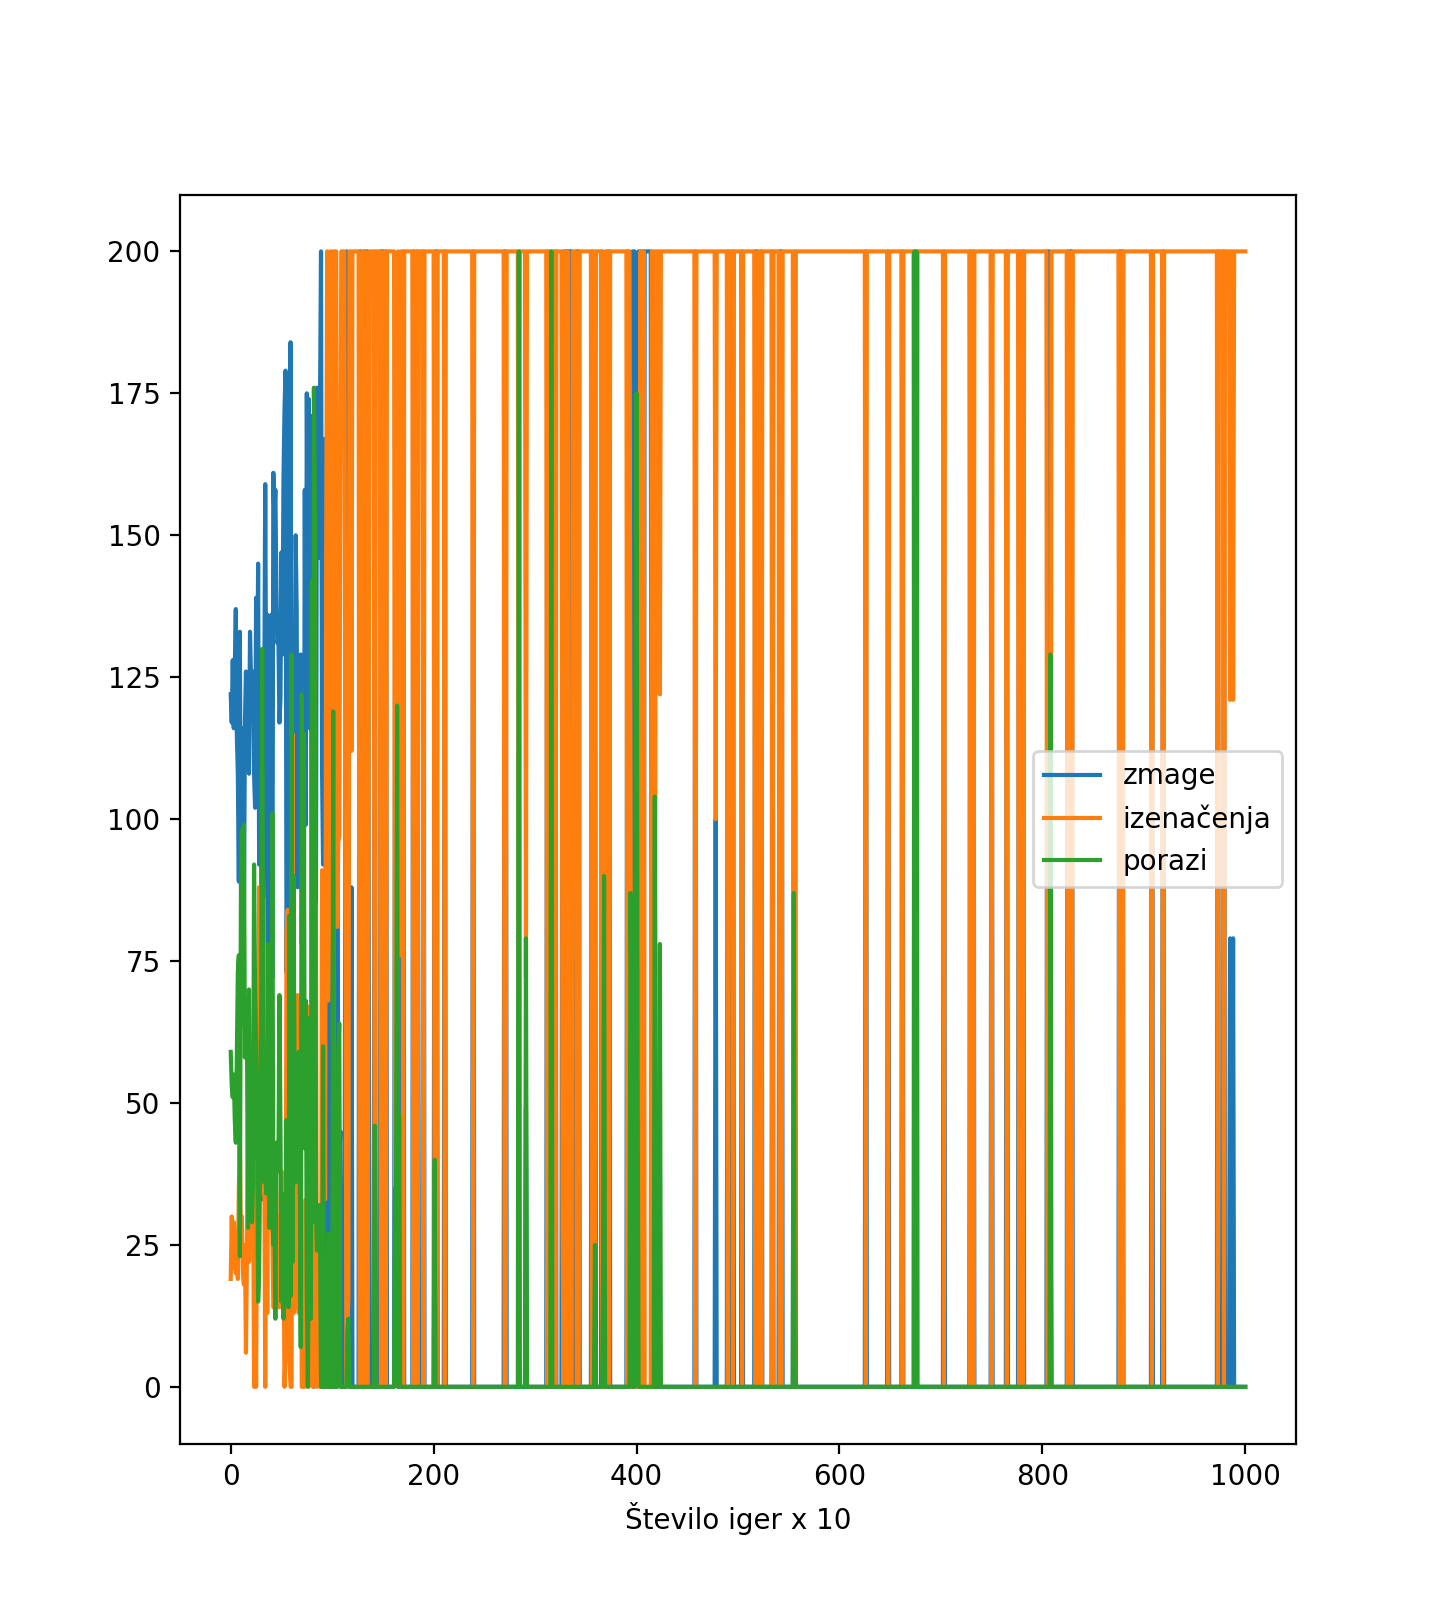
\includegraphics[scale=0.29]{slike/td-bulsit.png}
        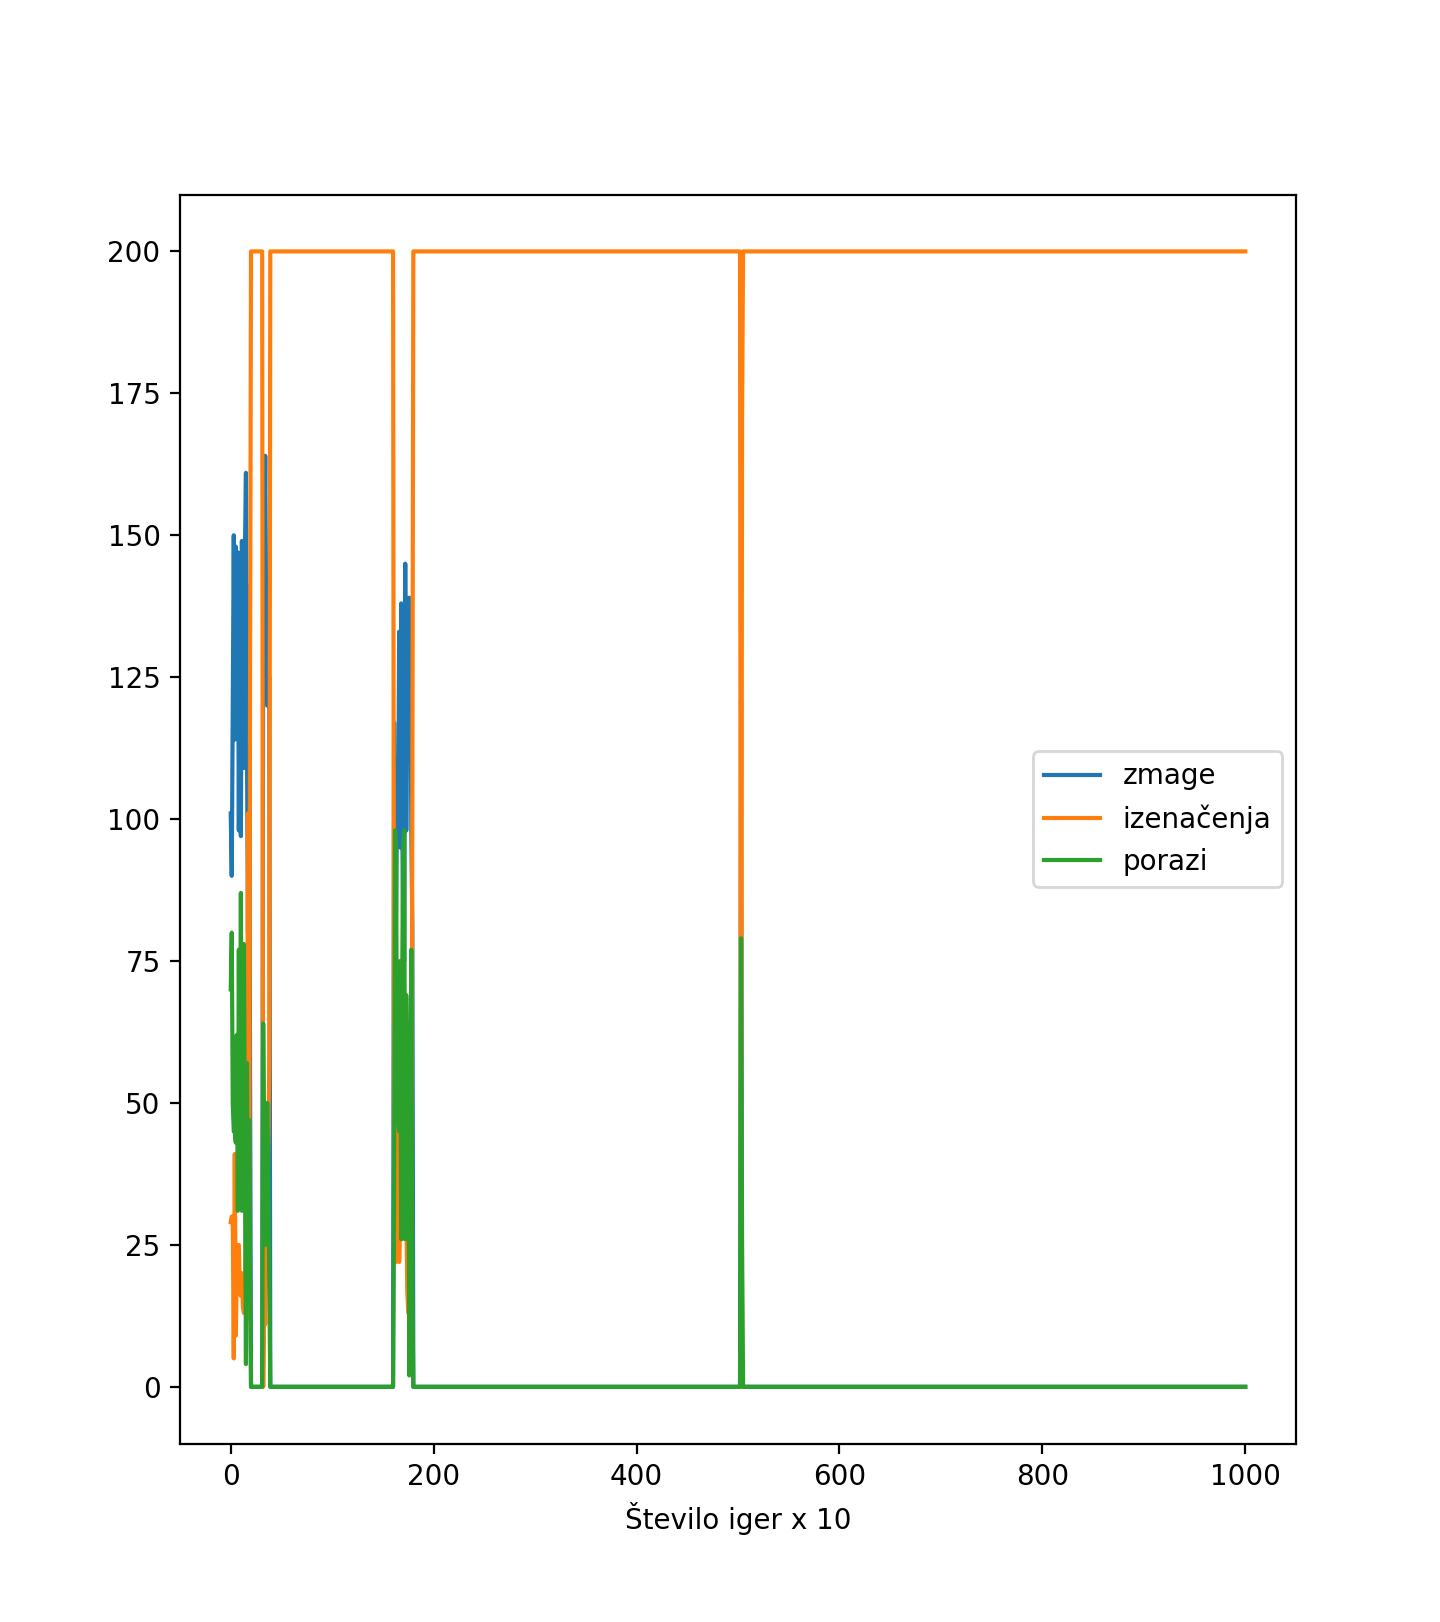
\includegraphics[scale=0.29]{slike/semi-razumljiv-agent.png}
    \end{figure}
\end{frame}


\begin{frame}
    \frametitle{4,4,3-igra}
    \begin{figure}
        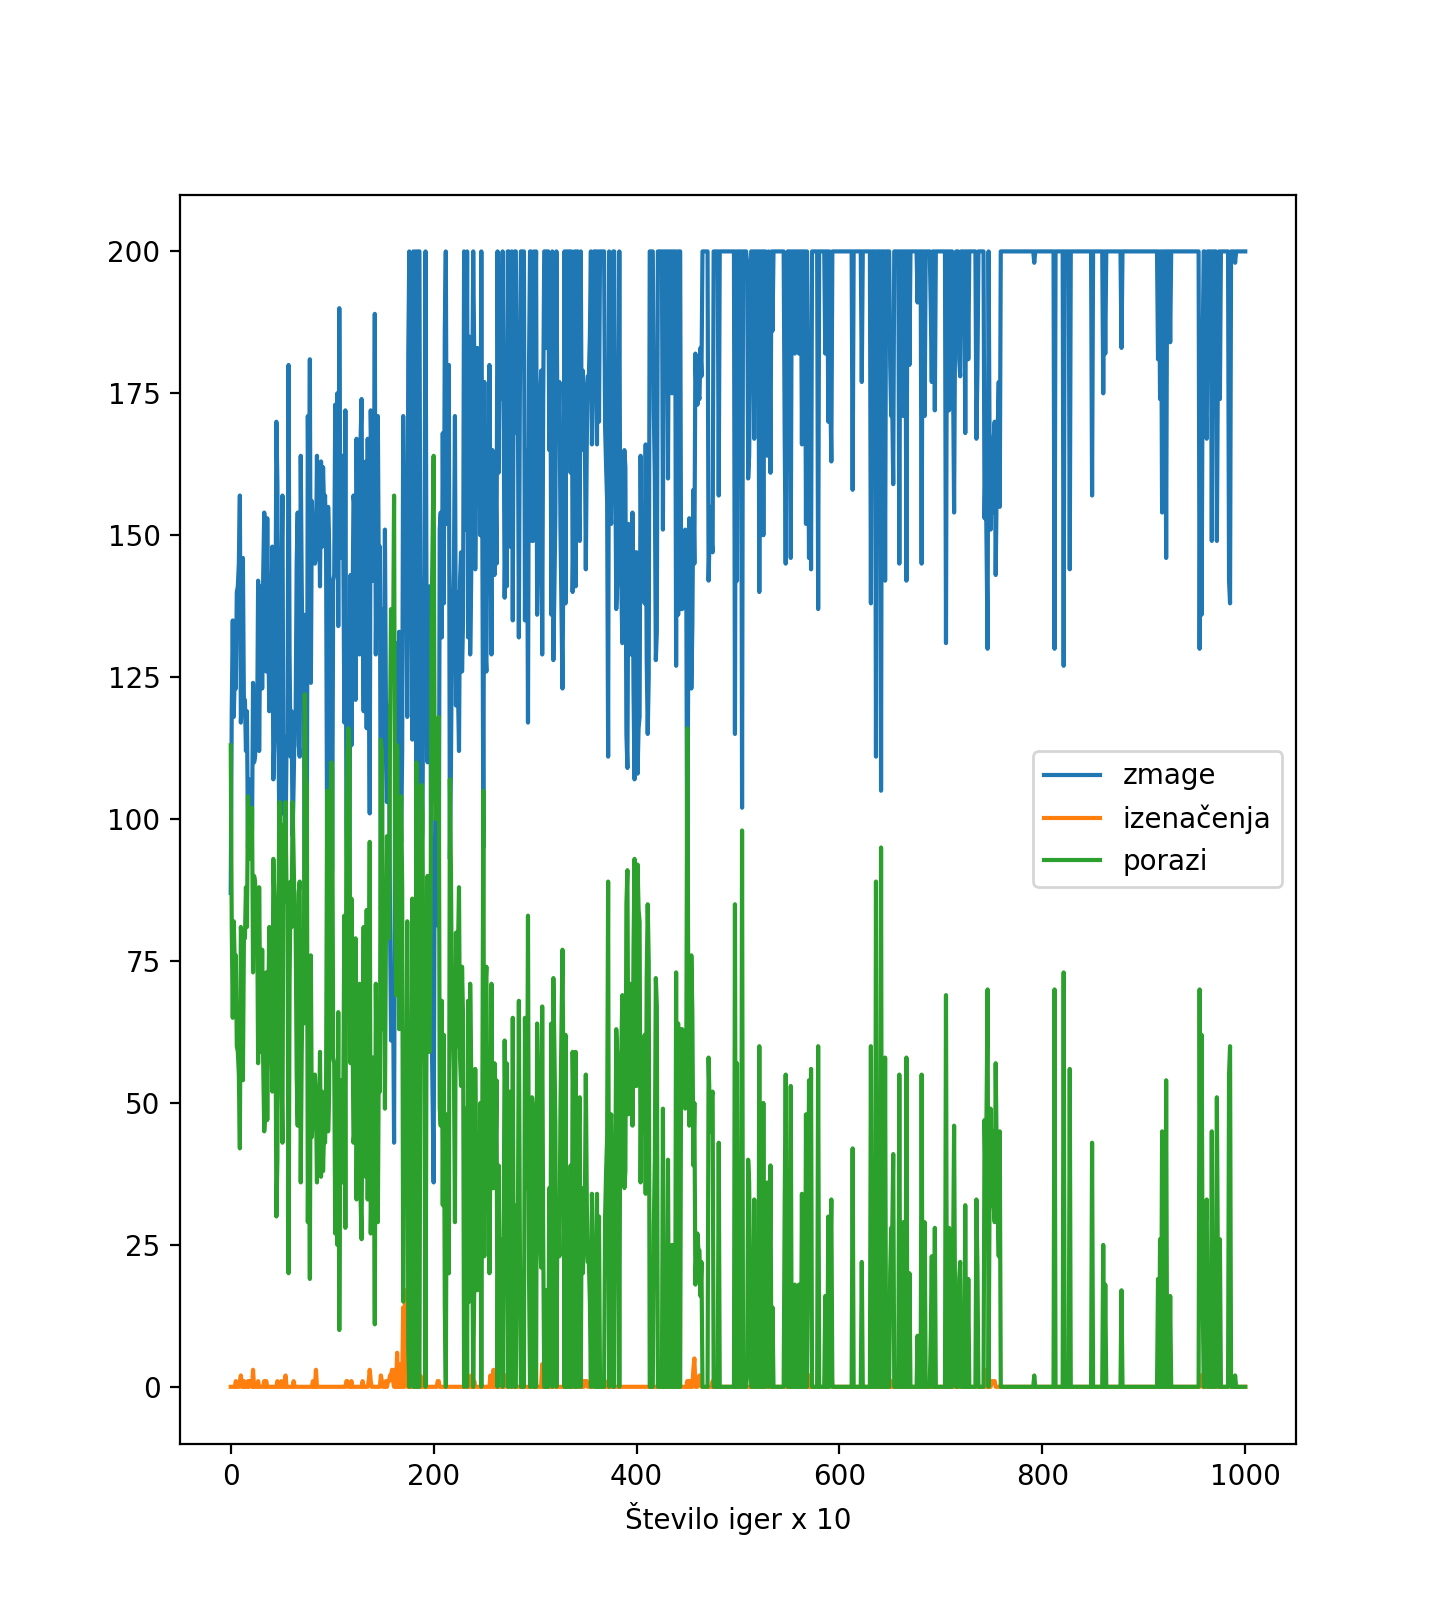
\includegraphics[scale=0.29]{slike/443-agent.png}
        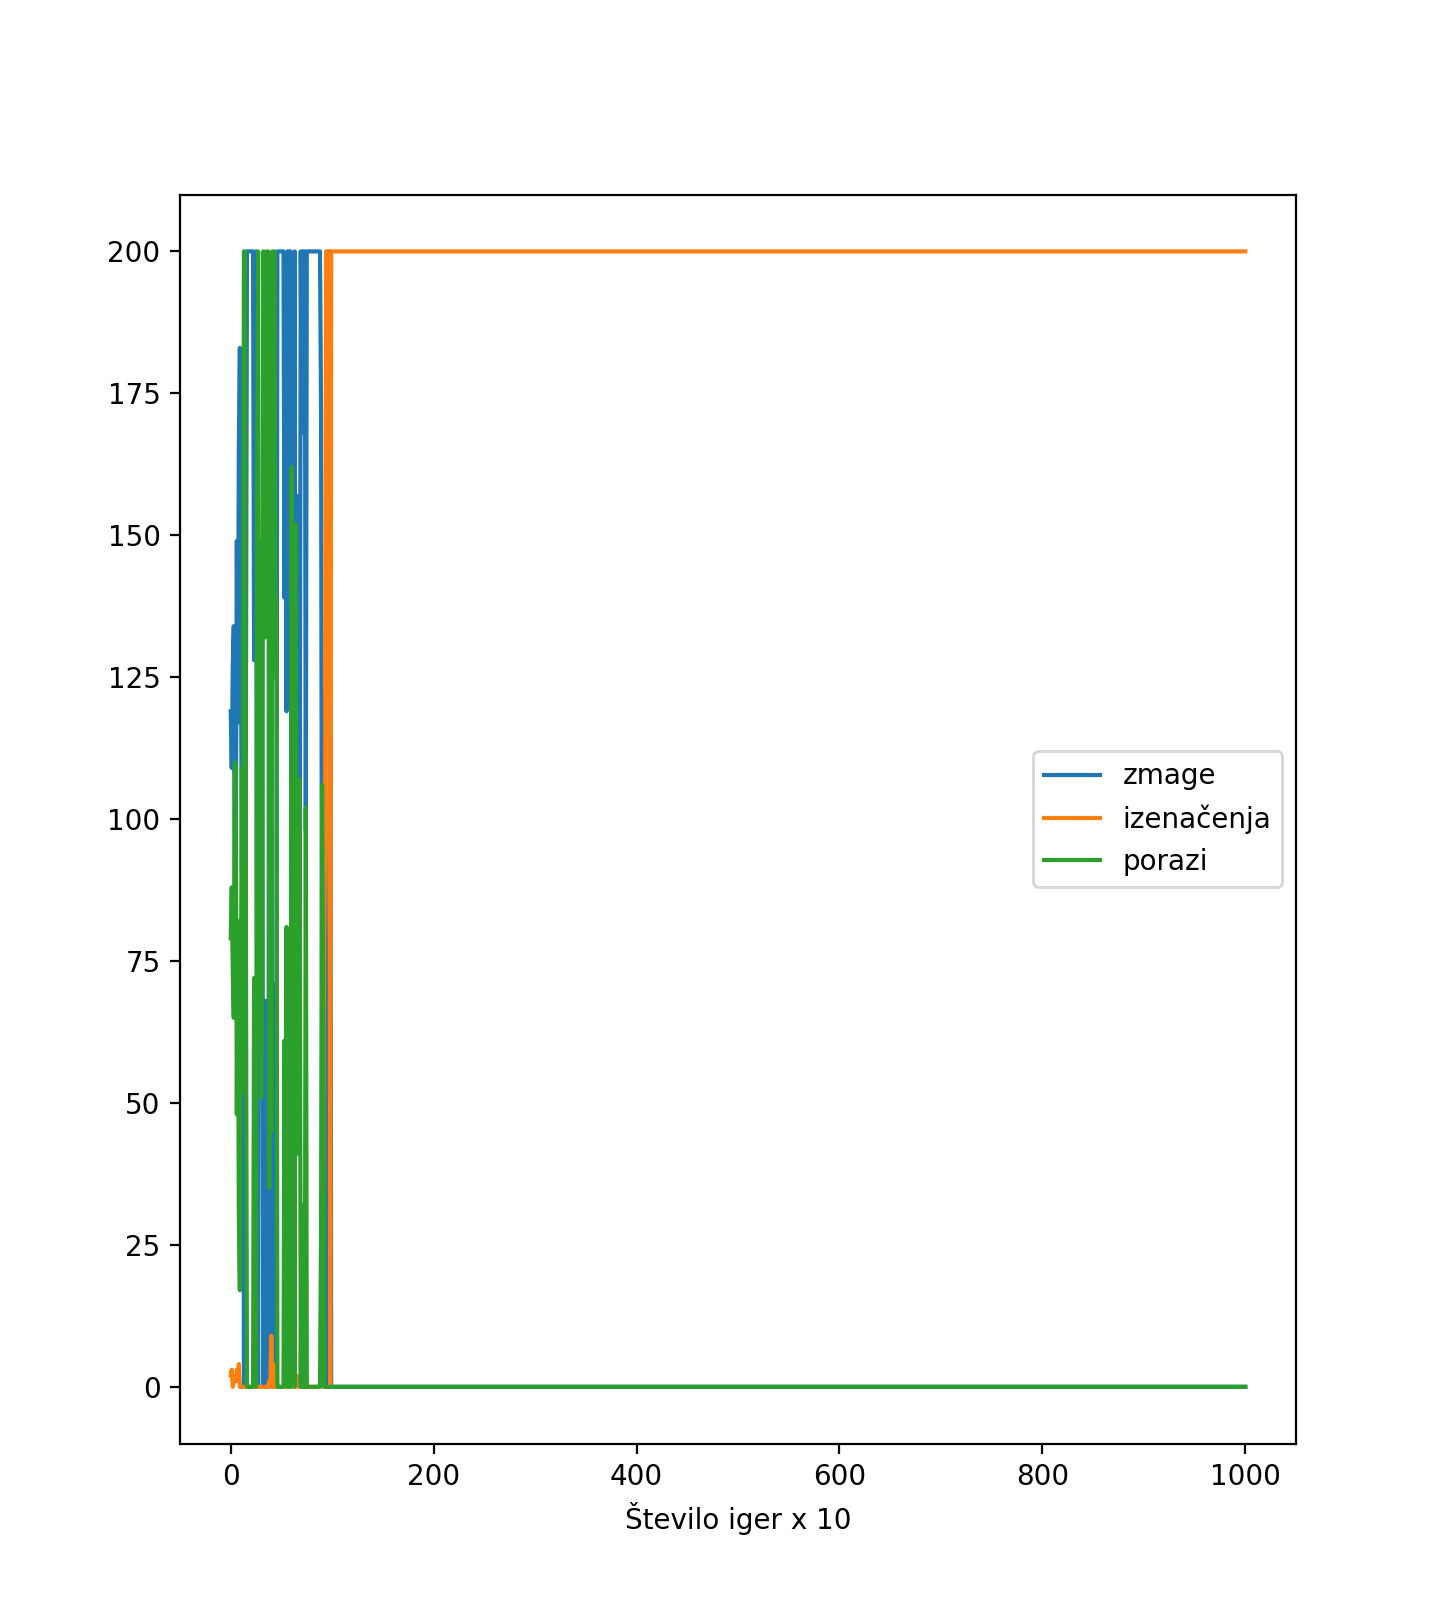
\includegraphics[scale=0.29]{slike/443g-agent.png}
    \end{figure}
\end{frame}


\begin{frame}
    \frametitle{4,4,4-igra}
    \begin{figure}
        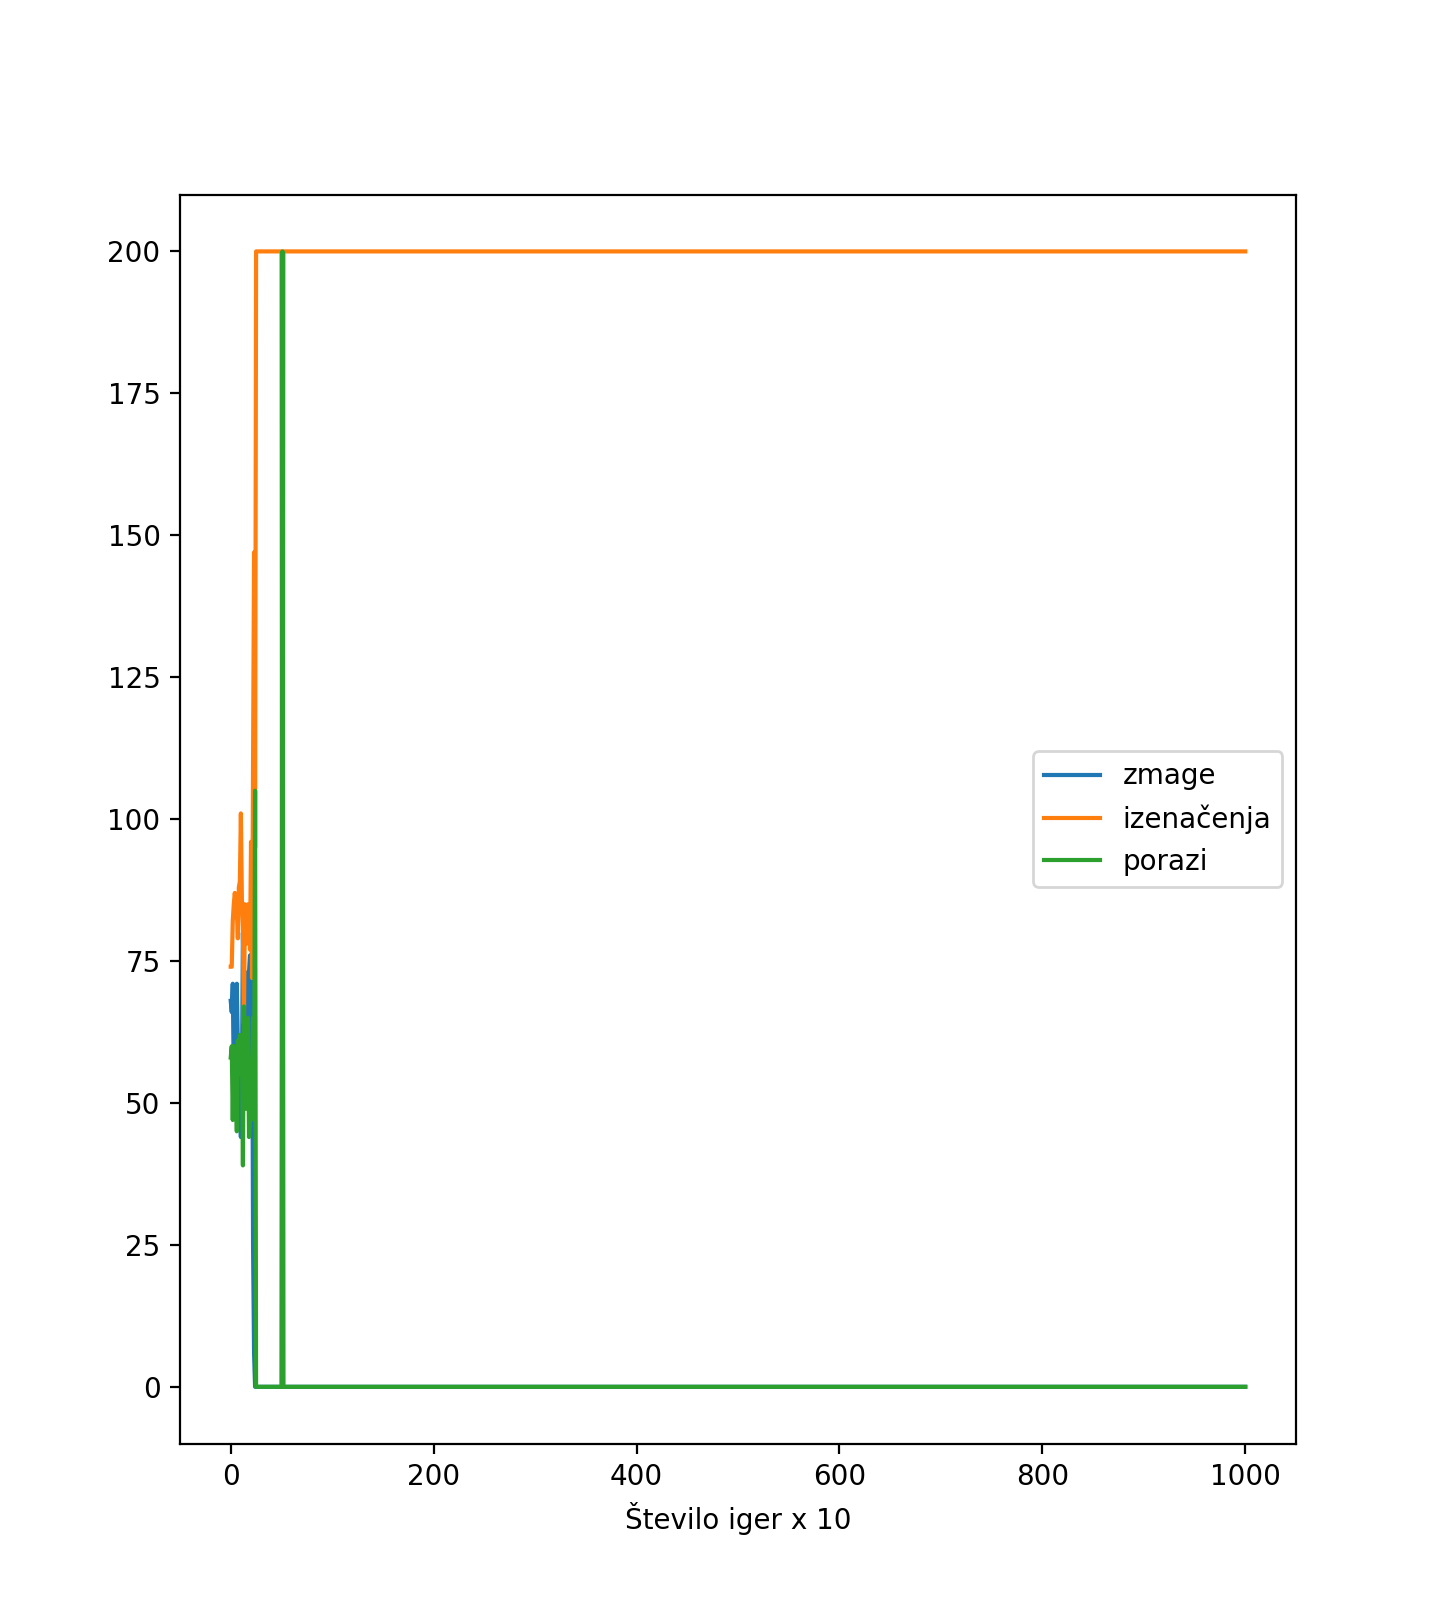
\includegraphics[scale=0.29]{slike/444-agent.png}
        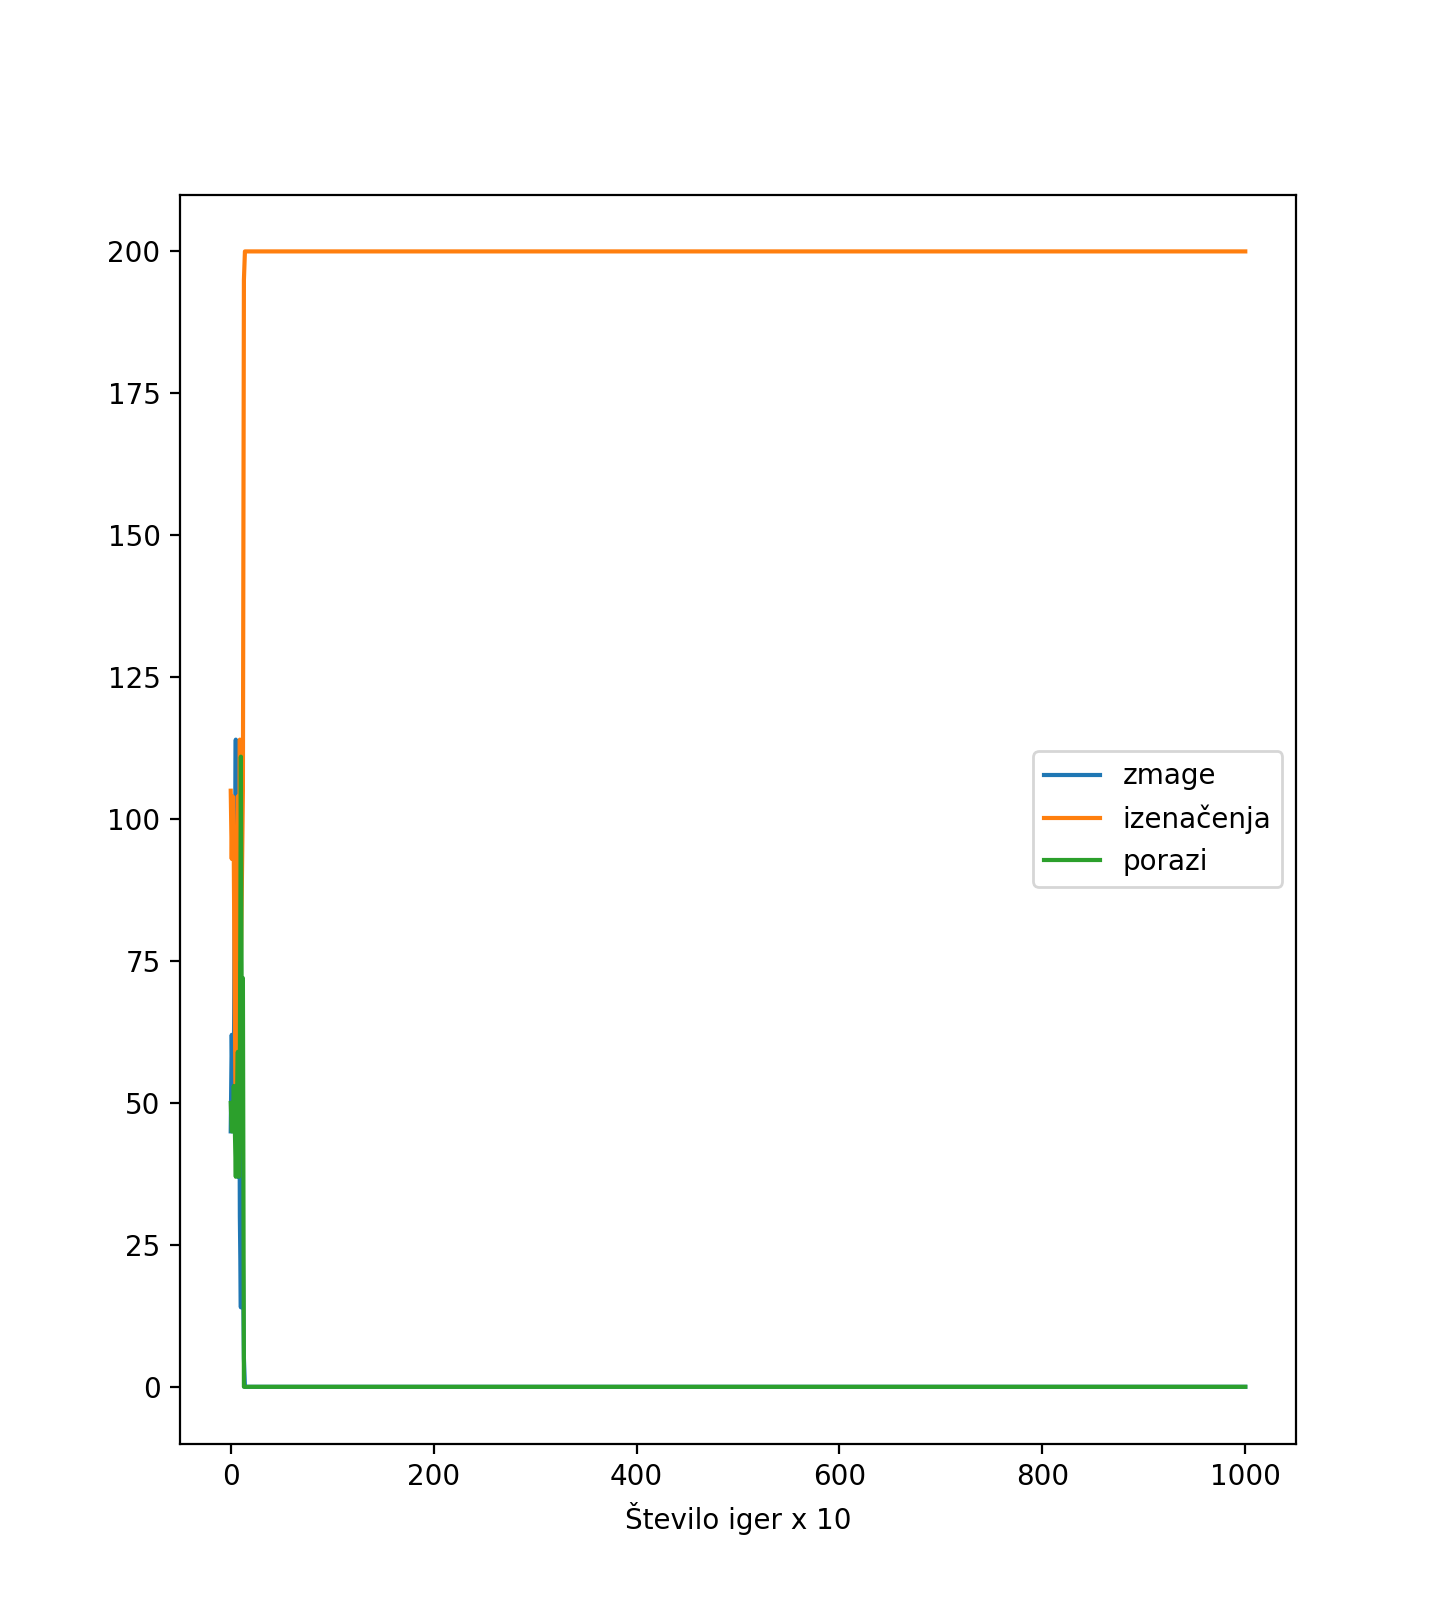
\includegraphics[scale=0.29]{slike/444g-agent.png}
    \end{figure}
\end{frame}


\begin{frame}
    \frametitle{5,5,4-igra}
    \begin{figure}
        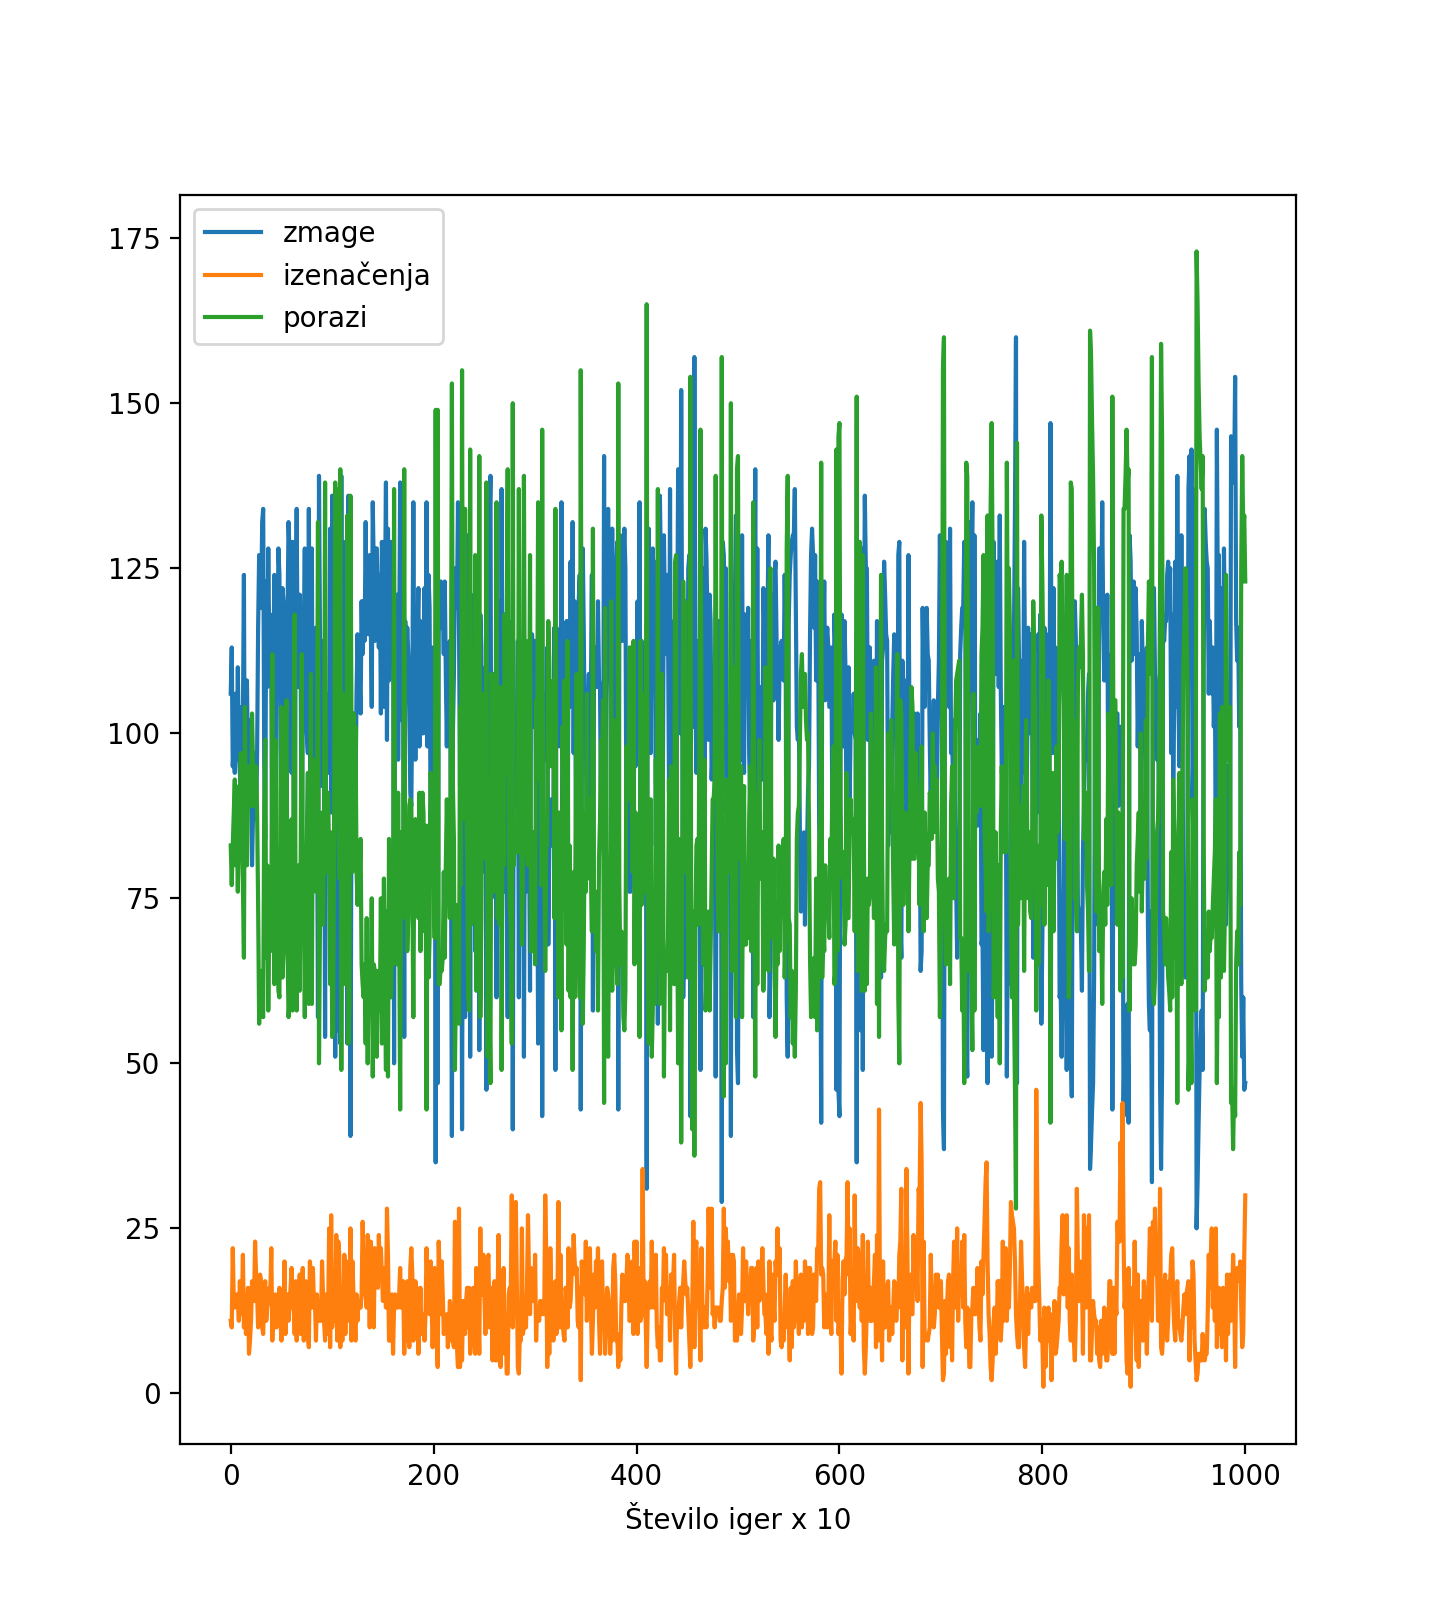
\includegraphics[scale=0.29]{slike/554-agent.png}
        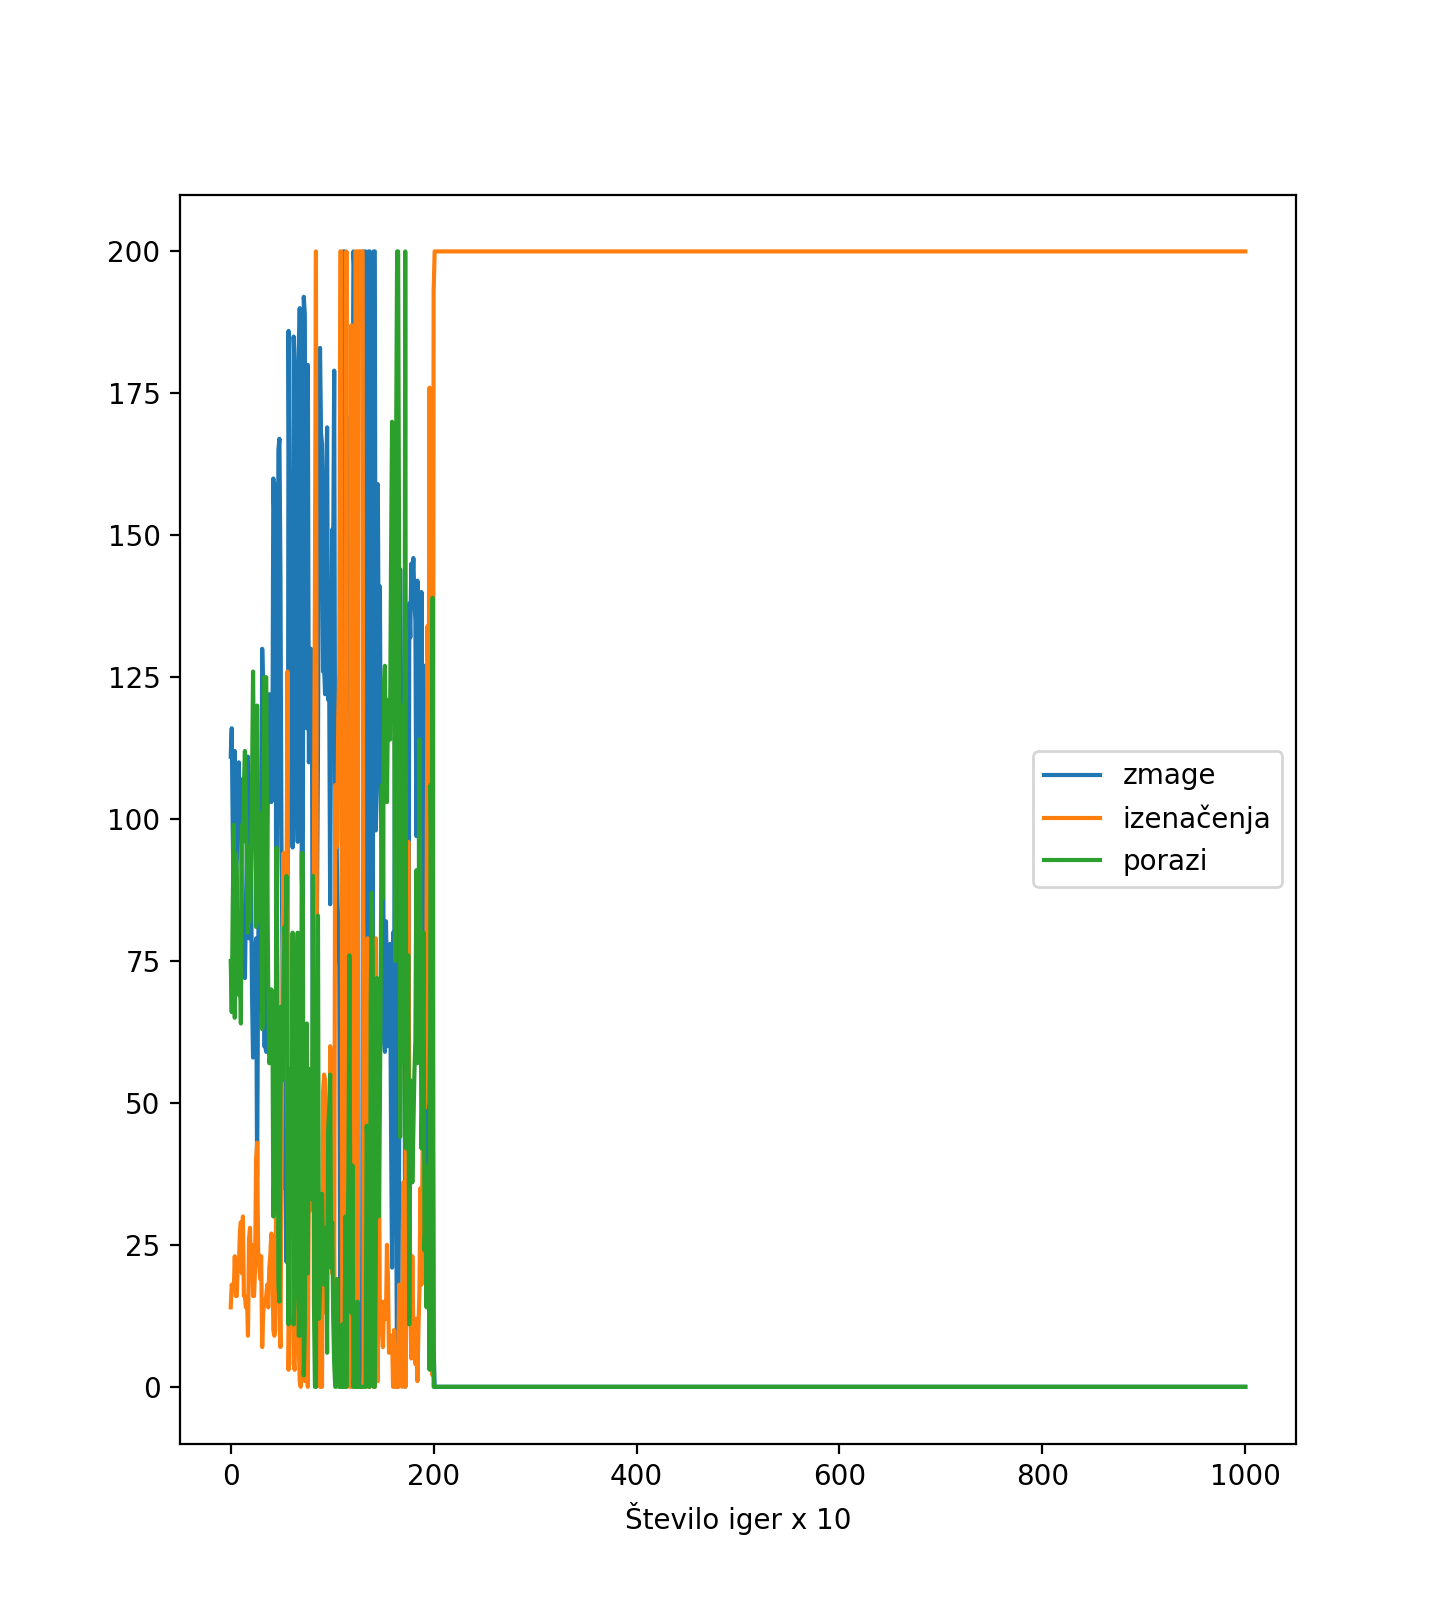
\includegraphics[scale=0.29]{slike/554g-agent.png}
    \end{figure}
\end{frame}


\begin{frame}[t, allowframebreaks]
    \frametitle{Literatura}
    \nocite{*}
    \bibliographystyle{plain}
    \bibliography{literatura}
\end{frame}


\end{document}
